\documentclass{article}

% if you need to pass options to natbib, use, e.g.:
%     \PassOptionsToPackage{numbers, compress}{natbib}
% before loading neurips_2026

% The authors should use one of these tracks.
% Before accepting by the NeurIPS conference, select one of the options below.
% 0. "default" for submission
% \usepackage{neurips_2026}
% \usepackage[eandd]{neurips_2026}
% the "default" option is equal to the "main" option, which is used for the Main Track with double-blind reviewing.
% 1. "main" option is used for the Main Track
%  \usepackage[main]{neurips_2026}
% 2. "position" option is used for the Position Paper Track
%  \usepackage[position]{neurips_2026}
% 3. "eandd" option is used for the Evaluations & Datasets Track
 \usepackage[eandd]{neurips_2026}
% 4. "creativeai" option is used for the Creative AI Track
%  \usepackage[creativeai]{neurips_2026}
% 5. "sglblindworkshop" option is used for the Workshop with single-blind reviewing
 % \usepackage[sglblindworkshop]{neurips_2026}
% 6. "dblblindworkshop" option is used for the Workshop with double-blind reviewing
%  \usepackage[dblblindworkshop]{neurips_2026}

\usepackage{amssymb}
\newcommand{\cmark}{\checkmark}
\newcommand{\xmark}{$\times$}
\usepackage{subcaption}
\usepackage{graphicx}
\usepackage{float}
% After being accepted, the authors should add "final" behind the track to compile a camera-ready version.
% 1. Main Track
 % \usepackage[main, final]{neurips_2026}
% 2. Position Paper Track
%  \usepackage[position, final]{neurips_2026}
% 3. Evaluations & Datasets Track
 % \usepackage[eandd, final]{neurips_2026}
% 4. Creative AI Track
%  \usepackage[creativeai, final]{neurips_2026}
% 5. Workshop with single-blind reviewing
%  \usepackage[sglblindworkshop, final]{neurips_2026}
% 6. Workshop with double-blind reviewing
%  \usepackage[dblblindworkshop, final]{neurips_2026}
% Note. For the workshop paper template, both \title{} and \workshoptitle{} are required, with the former indicating the paper title shown in the title and the latter indicating the workshop title displayed in the footnote.
% For workshops (5., 6.), the authors should add the name of the workshop, "\workshoptitle" command is used to set the workshop title.
% \workshoptitle{WORKSHOP TITLE}

% "preprint" option is used for arXiv or other preprint submissions
 % \usepackage[preprint]{neurips_2026}

% to avoid loading the natbib package, add option nonatbib:
%    \usepackage[nonatbib]{neurips_2026}

\usepackage[utf8]{inputenc} % allow utf-8 input
\usepackage[T1]{fontenc}    % use 8-bit T1 fonts
\usepackage{hyperref}       % hyperlinks
\usepackage{url}            % simple URL typesetting
\usepackage{booktabs}       % professional-quality tables
\usepackage{amsfonts}       % blackboard math symbols
\usepackage{nicefrac}       % compact symbols for 1/2, etc.
\usepackage{microtype}      % microtypography
\usepackage{xcolor}         % colors
\usepackage{amsmath} 
% Note. For the workshop paper template, both \title{} and \workshoptitle{} are required, with the former indicating the paper title shown in the title and the latter indicating the workshop title displayed in the footnote. 
\title{MIBE: Multi-subject Interaction Benchmark and Evaluator for Personalized Image Generation}


% The \author macro works with any number of authors. There are two commands
% used to separate the names and addresses of multiple authors: \And and \AND.
%
% Using \And between authors leaves it to LaTeX to determine where to break the
% lines. Using \AND forces a line break at that point. So, if LaTeX puts 3 of 4
% authors names on the first line, and the last on the second line, try using
% \AND instead of \And before the third author name.


\author{%
    Zhihan Chen\thanks{Equal contribution}\\
    University of California, Los Angeles\\
    % Los Angeles, CA 90095\\
    \texttt{chenz23@ucla.edu}\\
    \AND
    Yuhuan Zhao\footnotemark[1]\\
    University of Southern California\\
    % Los Angeles, CA 90007\\
    \texttt{yuhuanzh@usc.edu}\\
    \AND
    Yijie Zhu\footnotemark[1]\\
    DeerLab LLC\\
    % Mountain View, CA 94043\\
    \texttt{ ejzhu2025@gmail.com}\\
    \AND
    Xinyu Yao\footnotemark[1] \\
    Carnegie Mellon University\\
    % Pittsburgh, PA 15213 \\
    \texttt{xinyuyao@andrew.cmu.edu} \\
    \AND
    Mengcong Ren\\
    Clemson University\\
    % Clemson, SC 29634\\
    \texttt{mengcongren@gmail.com}
    \AND
    Suwen Wang\\
    University of California, Los Angeles\\
    \AND
    Qiuyang Yin\\
    Google\\
    \texttt{davidyqy@google.com}
    \AND
    Yuchen Sun\\
    San Jose State University\\
    \AND
    Qin Wang\\
    University of Illinois at Urbana-Champaign\\
    \AND 
    Lu Xin\\
    DeerLab LLC\\
    \texttt{lucasxinlu@outlook.com}
  % examples of more authors
  % \And
  % Coauthor \\
  % Affiliation \\
  % Address \\
  % \texttt{email} \\
  % \AND
  % Coauthor \\
  % Affiliation \\
  % Address \\
  % \texttt{email} \\
  % \And
  % Coauthor \\
  % Affiliation \\
  % Address \\
  % \texttt{email} \\
  % \And
  % Coauthor \\
  % Affiliation \\
  % Address \\
  % \texttt{email} \\
}


\begin{document}


\maketitle


\begin{abstract}
Multi-subject personalized image generation requires the precise rendering of all requested reference identities and their specified interactions based on a guiding prompt. However, state-of-the-art models still struggle with this process, frequently omitting subjects, failing to preserve reference appearances, or misattributing interactions. Furthermore, existing metrics designed primarily for single-subject fidelity cannot reliably capture these errors, suffering severe degradation in ranking separability and failing to align with human preference as the subject count increases. To address this gap, we introduce Multi-subject Interaction Benchmark and Evaluator (MIBE), a unified framework comprising a Multi-subject Interaction Benchmark (MIB) and a Multi-subject Interaction Evaluator (MIE). MIB systematically covers diverse relation types and scene complexities through a decoupled data regime. This consists of a 60K-pair VLM-labeled Silver Set for scalable metric training and a 4K-pair double-blind Human Evaluation Gold Set covering a diverse range of state-of-the-art generators. To demonstrate the utility of this benchmark, we present MIE, a lightweight, reference-conditioned evaluator trained exclusively on the Silver Set with a dual-head ranking and diagnosis objective. MIE exhibits strong cross-generator generalization on the Gold Set and achieves a significantly higher correlation with human preference. By outperforming a broad spectrum of baseline metrics, including CLIP and DINO variants, MIE demonstrates that diagnostic supervision can preserve ranking separability and human alignment where traditional evaluators collapse. Ultimately, by providing data with the diagnostic and preference labels required to train robust evaluators, MIBE serves as a comprehensive framework to benchmark multi-subject image generation and guide future model alignment.
\end{abstract}

\section{Introduction}

State-of-the-art personalized image generators can faithfully render a single reference identity, but as soon as a second subject is introduced---let alone four or eight---the generated image often contains the right scene, the right colors, and the wrong subjects. A model conditioned on reference photos of a specific child and a specific dog, asked to depict the child playing with the dog, may instead produce a generic child with a different dog, two children and no dog, or the right child standing beside an empty patch of grass. These are not merely aesthetic flaws; they are \emph{binding} failures, and they are largely invisible to current metrics.

We call this the \emph{binding} problem: every requested reference subject must (1) appear in the generated image (\emph{Existence}), (2) preserve its reference appearance without leakage from other subjects (\emph{Appearance}), and (3) participate in the prompt-specified role, relation, or object assignment (\emph{Interaction}). These dimensions are coupled: a missing subject often causes the model to redistribute its visual features onto surviving subjects, making appearance corruption a downstream consequence of existence failure (Section~\ref{sec:appendix_failure_modes}). The problem is especially fragile in contact-rich and occlusion-heavy scenes, where local evidence is ambiguous. Prior stress-test evaluation has documented this ``illusion of scalability,'' showing identity collapse in dense scenes while global CLIP-based scores remain misleadingly stable~\cite{chen2026identities}; MIBE complements that curated identity-collapse stress test with human-grounded labels, factorized binding stress, and a learned evaluator.

Existing automatic metrics are fragmented. CLIP- and DINO-based reference similarity captures appearance overlap but cannot verify which subject participates in which interaction. General preference models such as PickScore~\cite{kirstain2023pick}, ImageReward~\cite{xu2023imagereward}, and HPS~\cite{wu2023human} can favor visually polished but compositionally broken images. As Figure~\ref{fig:metric_agreement_subject_count} shows, as subject count grows from 2 to 8, the pairwise agreement of standard metrics with double-blind human judgment drops toward random choice. Existing benchmarks are similarly under-equipped, focusing on single-subject fidelity~\cite{ruiz2023dreambooth,peng2024dreambench}, text-only composition~\cite{huang2023t2i}, or broad multi-subject capability~\cite{chen2025xverse,wang2025psr}, without factorizing the conditions that induce binding failures. Binding is therefore both a generation and a measurement bottleneck.

\begin{figure}[t]
  \centering
  
\includegraphics[width=0.95\linewidth]{figures/section_4_2_1_baseline_alignment.png}
  \caption{
  \textbf{Existing metrics approach random agreement as subject count grows; MIE retains higher human alignment.}
  Pairwise agreement with double-blind human preference on MIB-Gold by subject count ($N \in \{2,4,6,8\}$). Standard metrics, including SCR~\cite{chen2026identities}, approach random agreement (dashed line) in high-subject-count settings; MIE, trained exclusively on MIB-Silver, retains higher agreement, with the gap widening as scenes grow more crowded.
  }
  \label{fig:metric_agreement_subject_count}
\end{figure}

We address this gap with \textbf{MIBE}, a unified framework that couples a \textbf{Multi-subject Interaction Benchmark (MIB)} with a learned \textbf{Multi-subject Interaction Evaluator (MIE)}. MIB adopts a silver--gold design: MIB-Silver provides 60K Nano Banana/MOSAIC candidate pairs labeled by SOP-guided dual-VLM consensus for scalable supervision, while MIB-Gold provides 4,020 double-blind human-labeled pairs across six generators for human-grounded evaluation. The benchmark uses hierarchical prompts over $N \in \{2,4,6,8\}$ subjects and factorizes binding stress by subject count, human/object composition, and relation type. This design supports both seen-generator validation on Nano Banana/MOSAIC and unseen-generator transfer to GPT-Image-1.5, Flux2, Seedream~4.5, and GLM.

\textbf{MIE} is trained exclusively on MIB-Silver and evaluated on MIB-Gold. 
Given the reference set, prompt, and candidate image, it jointly predicts a pairwise ranking score and Existence/Appearance/Interaction diagnostics. 
MIE consistently outperforms baseline metrics in agreement with double-blind human judgment, with the gap widening as subject count scales from 2 to 8.

In summary, this paper makes three contributions:
\begin{itemize}
    \setlength{\itemsep}{2pt}
    \setlength{\parskip}{0pt}
    \setlength{\parsep}{0pt}

    \item We introduce \textbf{MIB}, a controlled benchmark for reference-conditioned multi-subject generation that factorizes subject count, human/object composition, and relation type, with a 60K dual-VLM-consensus silver set and a 4{,}020-pair double-blind human-labeled gold set covering six state-of-the-art generators.
    \item We propose \textbf{MIE}, a reference-conditioned evaluator that jointly learns pairwise ranking and structured diagnostics over \emph{Existence}, \emph{Appearance}, and \emph{Interaction}, providing both human-aligned preference prediction and interpretable failure attribution.
    \item Through cross-generator meta-evaluation on MIB-Gold, we reveal systematic failure patterns---failure rates that scale with subject count, coupled Existence--Appearance failures, and interaction-induced subject deformation---providing actionable targets for future model alignment.
\end{itemize}

\section{Related Work}
\paragraph{Personalized and Multi-Subject Generation}
Personalized image generation has evolved from early optimization-based methods like DreamBooth \cite{ruiz2023dreambooth} and Textual Inversion \cite{gal2022image} to efficient encoder-based models such as IP-Adapter \cite{ye2023ip} and PhotoMaker \cite{li2024photomaker}. While effective for single subjects, these methods struggle with binding in multi-subject scenarios—ensuring each reference identity is correctly assigned to its specific role and attributes. Recent works like FastComposer \cite{xiao2023fastcomposer}, MS-Diffusion \cite{wang2024ms}, and Interact-Custom \cite{xu2025interactcustom} address this through localized attention and identity decoupling. However, a significant measurement gap remains: existing methods are rarely tested in contact-rich or occlusion-heavy tasks regimes where subjects overlap, leading to frequent failures in physical grounding and identity leakage that current metrics fail to capture.

\paragraph{Evolution of Benchmark}
While compositional benchmarks like T2I-CompBench \cite{huang2023t2i} evaluate text-to-image alignment, they lack the reference conditioning necessary to measure identity preservation. Recent efforts such as XVerseBench \cite{chen2025xverse}, PSRBench \cite{wang2025psr}, and MultiHuman-Testbench \cite{borse2025multihuman} have introduced multi-subject evaluations, yet they primarily focus on subject count or spatial positioning. 
As summarized in Table~\ref{tab:benchmark_comparison}, MIB distinguishes itself by targeting relation-level binding. Unlike MultiBind \cite{tian2026multibind}, which explores attribute-level misbinding, MIB factorizes complex physical interactions and occlusions. It serves as both a diagnostic testbed and a training substrate, decoupling scalable "silver" supervision from human "gold" evaluation to provide a more granular view of how models handle locally ambiguous visual evidence.

\paragraph{Metrics and Scalable Evaluators}
Standard metrics often provide incomplete assessments of multi-subject quality: CLIP-based scores lack instance-specific grounding, while reward models like ImageReward \cite{xu2023imagereward} often prioritize aesthetics over logical binding. Although Vision-Language Models (VLMs) are increasingly used as automated judges, they remain sensitive to prompting and poorly calibrated for absolute scoring \cite{kumar2026vlmjudge}. MIBE addresses these limitations by adopting a pairwise ranking format and a latent scalar utility model, rather than absolute numeric ratings. By combining an "errors-first" VLM consensus for scalable MIB-Silver labels with human-verified MIB-Gold data, MIBE unifies preference learning with structured diagnostic supervision for more robust, reference-grounded evaluation.


% \paragraph{Personalized Image Generation}
% Personalized image generation aims to synthesize images that preserve the appearance of reference subjects while following a target prompt. Early methods such as Textual Inversion~\cite{gal2022image}, DreamBooth~\cite{ruiz2023dreambooth}, and Custom Diffusion~\cite{kumari2023multi} personalize diffusion models through token learning or model adaptation. More recent encoder-based methods, including IP-Adapter~\cite{ye2023ip}, InstantID~\cite{wang2024instantid}, and PhotoMaker~\cite{li2024photomaker}, amortize personalization through feed-forward reference conditioning. These methods substantially improve efficiency and single-subject fidelity, but are primarily studied in settings where one dominant subject, or a small number of visually separable concepts, must be preserved.

% Multi-subject personalization introduces a harder problem: \emph{binding}. Each reference subject must be assigned to the correct generated instance, visual attributes, and prompt-specified role. Recent methods such as FastComposer~\cite{xiao2023fastcomposer}, Mix-of-Show~\cite{gu2023mix}, MS-Diffusion~\cite{wang2024ms}, MuDI~\cite{jang2024mudi}, UniPortrait~\cite{he2024uniportrait}, AnyStory~\cite{he2025anystory}, MOSAIC~\cite{she2025mosaic}, XVerse~\cite{chen2025xverse}, RealCustom++~\cite{realcustom2024}, FocusDPO~\cite{jin2025focusdpo}, and PSR~\cite{wang2025psr} address multi-concept or multi-subject composition through localized attention, routing, identity decoupling, disentanglement, architecture-specific modulation, or preference optimization. Interact-Custom~\cite{xu2025interactcustom} further highlights customized human-object interaction as an important generation setting where identity preservation and interaction control must be handled jointly.

% However, progress on generation methods exposes a measurement gap. Existing evaluations still provide limited systematic evidence in contact-rich and occlusion-heavy regimes, where subjects are no longer visually separable. Dense physical interactions, partial occlusions, shared objects, and overlapping body regions can expose failures that are not fully captured by standard identity-similarity or subject-consistency metrics, including missing subjects, fused boundaries, appearance leakage, role confusion, and relation misassignment. Our focus is therefore not merely whether multiple references can be rendered together, but whether each reference remains correctly bound to its generated instance, appearance, prompt-specified role, and interaction target when visual evidence becomes locally ambiguous. In this sense, robust benchmark infrastructure is a prerequisite for further progress: without binding-diagnostic supervision and human-grounded evaluation, methods optimized for narrow identity or consistency objectives may improve aggregate scores while still failing at relation-level grounding.

% \paragraph{Benchmarks for Personalized and Compositional Generation} 
% Existing benchmarks capture only part of this problem. Text-only compositional benchmarks such as T2I-CompBench~\cite{huang2023t2i} evaluate attribute, object, and spatial alignment, but they do not provide reference images and therefore cannot measure identity preservation, identity collapse, or appearance leakage. Personalized generation benchmarks such as DreamBench~\cite{ruiz2023dreambooth}, DreamBench++~\cite{peng2024dreambench}, and CustomConcept101~\cite{kumari2023multi} introduce reference-conditioned evaluation, but mainly focus on single-subject or limited multi-concept settings rather than systematic multi-subject interaction and occlusion stress.

% Recent benchmarks move closer to reference-conditioned multi-subject evaluation. XVerseBench~\cite{chen2025xverse} evaluates single-, dual-, and triple-subject personalized generation. Concurrent PSRBench~\cite{wang2025psr} provides a broad capability-oriented benchmark over attributes, backgrounds, actions, positions, complex prompts, and three- or four-subject generation. OmniContext~\cite{wu2025omnigen2} evaluates in-context generation across characters, objects, and scenes, while MultiBanana~\cite{oshima2025multibanana} studies multi-reference text-to-image generation under reference-count variation and other multi-reference-specific challenges. MultiHuman-Testbench~\cite{borse2025multihuman} focuses on multi-human generation with face identity, action, and prompt-alignment metrics. Concurrently, spatial benchmarks such as SpatialGenEval~\cite{spatialgeneval2026} systematically explore spatial intelligence and occlusion, but are confined to general text-to-image generation rather than reference-conditioned personalization.

% Most closely related to our binding motivation, MultiBind~\cite{tian2026multibind} studies cross-subject attribute misbinding in multi-reference, multi-subject generation, using slot-level correspondence and confusion-aware evaluation to expose drift, swap, dominance, and blending. MIB differs by targeting \emph{relation-level} binding rather than only attribute-level or slot-level misbinding. Specifically, MIB factorizes non-contact relations, occlusion, and physical interaction under reference conditioning, and evaluates whether the correct reference identities participate in the correct prompt-specified roles and interaction targets.

% MIB is designed to fill this missing benchmark regime and to support evaluator learning, not merely leaderboard-style comparison. Instead of treating multi-subject generation as simply ``more subjects in one image,'' MIB explicitly controls subject count, human/object composition, and relation type. It further decouples scalable silver supervision from human gold evaluation, allowing the benchmark to serve both as a controlled testbed for generator and metric comparison and as a training substrate for reference-conditioned evaluators. Table~\ref{tab:benchmark_comparison} summarizes how MIB differs from prior benchmarks.

\begin{table*}[t]
\centering
\scriptsize
\setlength{\tabcolsep}{3.0pt}
\renewcommand{\arraystretch}{1.12}
\resizebox{\textwidth}{!}{
\begin{tabular}{l c c c c c c p{3.2cm}}
\toprule
\textbf{Benchmark} 
& \textbf{Year}
& \textbf{Ref. Images} 
& \textbf{Multi-subj.} 
& \textbf{Stress / Eval. Design} 
& \textbf{Human Gold Eval.}
& \textbf{Pref./Diag. Supervision}
& \textbf{Main Gap} \\
\midrule

T2I-CompBench~\cite{huang2023t2i}
& 2023
& \xmark
& Text-only
& Text-only composition
& \xmark
& \xmark
& Cannot measure reference identity, identity collapse, or appearance leakage. \\

DreamBench~\cite{ruiz2023dreambooth}
& 2023
& \cmark
& \xmark
& Single-subject prompts
& \xmark
& \xmark
& No multi-subject binding or interaction evaluation. \\

DreamBench++~\cite{peng2024dreambench}
& 2024
& \cmark
& \xmark
& Single-subject, human-aligned automated eval.
& \xmark
& \xmark
& Broader single-subject evaluation, but no high-subject-count binding stress. \\

CustomConcept101~\cite{kumari2023multi}
& 2023
& \cmark
& Limited
& Multi-concept composition
& \xmark
& \xmark
& Not designed for contact-rich or occlusion-driven identity binding. \\

XVerseBench~\cite{chen2025xverse}
& 2025
& \cmark
& \cmark
& Single / dual / triple subjects
& \xmark
& \xmark
& Limited high-subject-count and relation-level stress factorization. \\

PSRBench~\cite{wang2025psr}
& 2025
& \cmark
& \cmark
& Broad capability subsets
& \xmark
& Reward metrics
& Capability-oriented; not a factorized diagnostic benchmark for interaction/occlusion binding failures. \\

OmniContext~\cite{wu2025omnigen2}
& 2025
& \cmark
& \cmark
& In-context character / object / scene eval.
& \xmark
& Automated judge scores
& Broad in-context consistency benchmark, but lacks human gold and factorized relation-level binding stress. \\

MultiBanana~\cite{oshima2025multibanana}
& 2025
& \cmark
& \cmark
& Multi-reference challenges
& \xmark
& VLM-based scores
& Covers multi-reference difficulty, but not hierarchical interaction/occlusion diagnosis or human pairwise gold labels. \\

MultiHuman-Testbench~\cite{borse2025multihuman}
& 2025
& \cmark
& \cmark
& Multi-human actions / faces
& \xmark
& Metric suite
& Restricted to human subjects; does not cover human-object or object-object binding. \\

MultiBind~\cite{tian2026multibind}
& 2026
& \cmark
& \cmark
& Attribute / slot misbinding
& \xmark
& Diagnostic metrics
& Focuses on attribute-level misbinding rather than factorized physical interaction and occlusion stress. \\

\midrule
\textbf{MIB (Ours)}
& \textbf{2026}
& \cmark
& \cmark
& \textbf{Factorized relation-level binding stress}
& \cmark
& \cmark
& -- \\

\bottomrule
\end{tabular}
}
\caption{Comparison with existing compositional and personalized generation benchmarks. DreamBench refers to the evaluation set introduced with DreamBooth, and CustomConcept101 refers to the concept set released with Custom Diffusion. Prior benchmarks mainly focus on text-only composition, single-subject personalization, broad multi-subject capability evaluation, multi-reference consistency, multi-human generation, or attribute-level misbinding. MIB targets reference-conditioned multi-subject personalization under factorized non-contact, occlusion, and physical-interaction stress, and provides both scalable preference/diagnostic supervision and human gold evaluation.}
\label{tab:benchmark_comparison}
\end{table*}

% \paragraph{Metrics and Scalable Evaluation}
% Existing metrics capture only partial projections of multi-subject personalization quality. Text-image metrics such as CLIP-T and SigLIP-T measure coarse prompt alignment and approximate subject existence, but cannot verify whether each generated instance matches the correct reference. Reference-image metrics such as CLIP-I, SigLIP-I, DINO-based similarities, and Detect-and-Compare-style subject metrics~\cite{jang2024mudi} are closer to appearance or identity evaluation, but global similarity can hide localized identity failures, while crop-based evaluation becomes unreliable under contact, occlusion, and overlapping subjects. Relation-oriented or VQA-style metrics, such as TIFA~\cite{hu2023tifa} and VQAScore / GenAI-Bench~\cite{lin2024vqascore}, improve compositional text-image evaluation, but they do not verify whether the correct reference identities participate in the correct relation.

% General preference and reward models, including ImageReward~\cite{xu2023imagereward}, PickScore~\cite{kirstain2023pick}, and HPS~\cite{wu2023human}, provide holistic assessments of realism, aesthetics, and prompt preference. MLLM-based explainable evaluators such as VIEScore~\cite{ku2024viescore} further demonstrate the potential of language-guided multimodal evaluation. However, these metrics are not calibrated for strict reference-grounded binding: a visually pleasing image may still contain missing subjects, identity swaps, appearance leakage, or incorrect interaction targets. Conversely, purely diagnostic binary checks cannot capture relative failure severity: two generations may both fail Existence or Interaction, yet differ substantially in how many subjects are missing or how severely relations are misassigned.

% To overcome the limitations of holistic reward models, recent paradigms increasingly adopt Vision-Language Models (VLMs) as automated judges. However, studies of MLLM/VLM-as-a-judge evaluation show that multimodal judges remain task-dependent and can be poorly calibrated for absolute scoring, while relative comparison is often more suitable than standalone numeric ratings~\cite{chen2024mllmjudge,kumar2026vlmjudge}. This ranking-scoring decoupling motivates a pairwise supervision format. MIBE avoids using standalone absolute numeric ratings as training targets; instead, MIE learns a latent scalar utility through pairwise comparisons, together with structured diagnostic prediction. Ranking captures which candidate is better overall, while diagnosis identifies whether failures arise from Existence, Appearance, or Interaction.

% Scalable evaluator training further requires supervision beyond small human-labeled sets. Large vision-language models can provide scalable annotations by inspecting references, prompts, and generated candidates together, but generic VLM preference prompting may over-weight aesthetics or global plausibility. MIBE therefore treats VLM labels as scalable but noisy supervision rather than final ground truth. MIB-Silver uses an errors-first SOP and cross-model consensus to obtain dense preference and diagnostic labels, while MIB-Gold reserves human annotations for final meta-evaluation of generators and learned evaluators.

% Taken together, prior work has advanced multi-subject generation and its evaluation, but existing benchmarks and metrics still do not jointly provide factorized interaction/occlusion stress, reference-grounded binding diagnosis, pairwise preference supervision, and human gold meta-evaluation. MIBE is designed to unify these components.

\section{Methods}
\subsection{MIB Construction}

\begin{figure}[t]
    \centering
    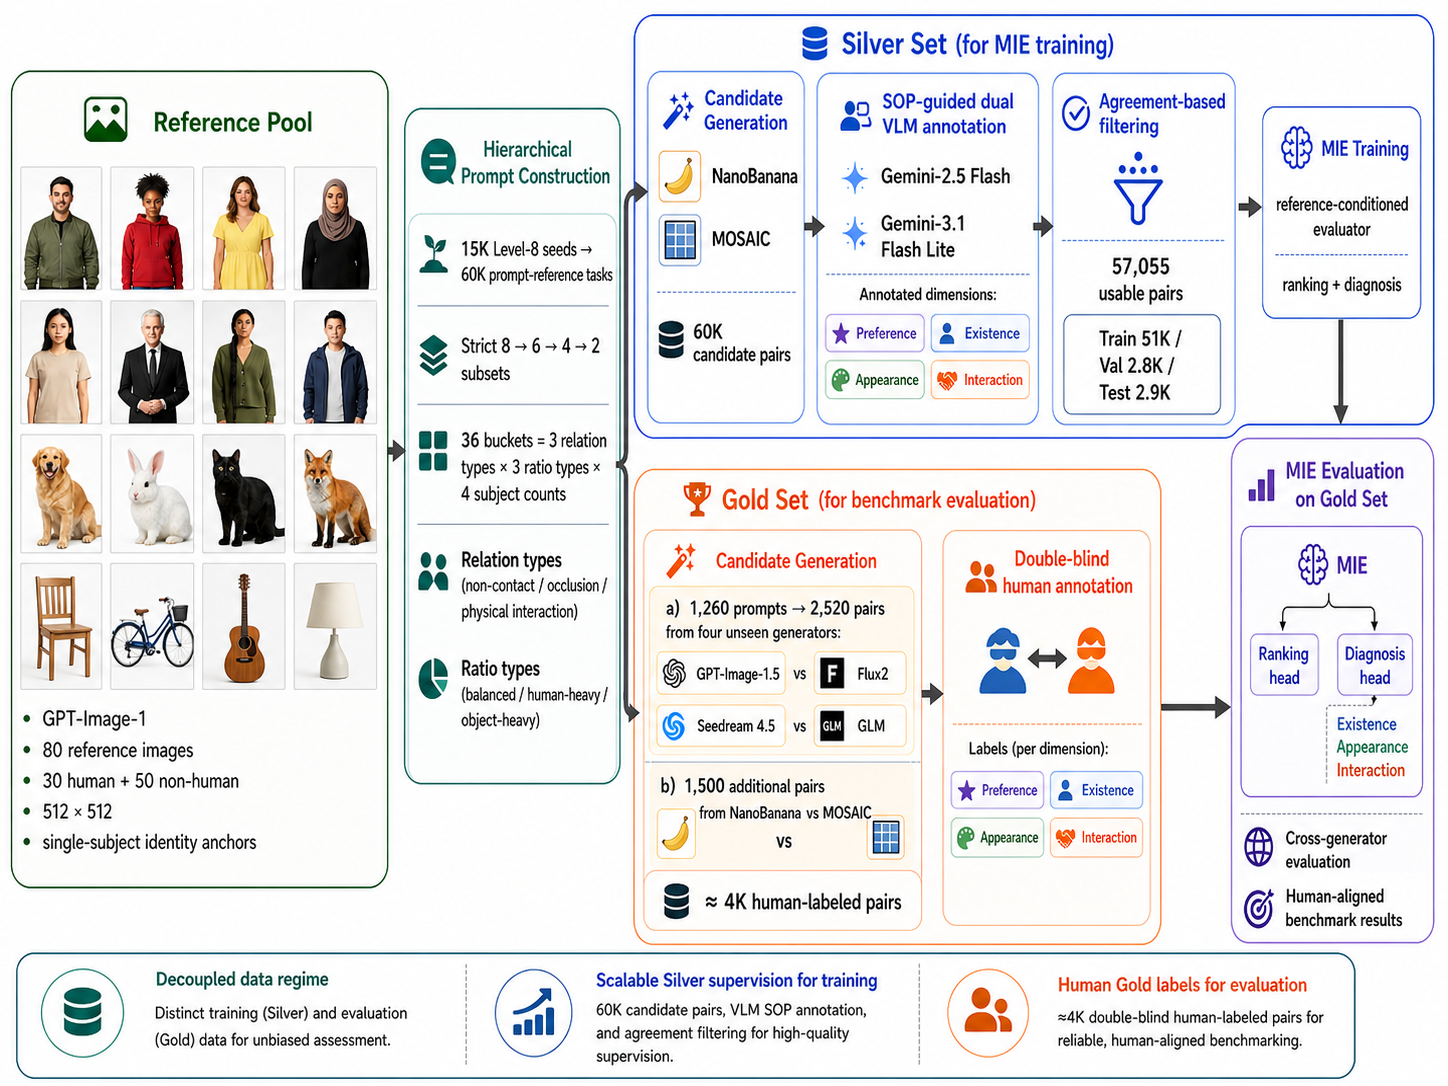
\includegraphics[width=0.95\linewidth,height=0.35\textheight]{mibe_overview.png}
    \caption{Overview of MIBE. The framework decouples reference construction, hierarchical prompt construction, candidate generation, and label acquisition. The Silver Set provides scalable SOP-guided VLM supervision for training MIE, while the Gold Set is double-blind human-labeled and reserved for benchmark evaluation.}
    \label{fig:mibe_construction}
\end{figure}

MIB is the data substrate of MIBE. It consists of controlled prompt-reference tasks, paired generated candidates, and their associated preference and diagnostic labels. Each task specifies a guiding prompt, a set of reference subjects, and two candidate generations produced under the same prompt-reference condition, enabling controlled comparison across subject counts, relation types, and generator outputs.

MIB follows a decoupled data regime that separates reference construction, prompt-task design, candidate generation, and label acquisition into independent stages. Reference images are constructed as single-subject identity anchors, while candidate images are generated as multi-subject interaction scenes under controlled prompt-reference conditions. This design allows subject identity, scene complexity, relation type, candidate generator, and annotation source to be controlled separately, reducing confounding factors in benchmark construction and enabling a clean separation between scalable evaluator training and human-centered benchmark evaluation.

\subsubsection{Prompt Construction}
\begin{figure*}[t]
    \centering
    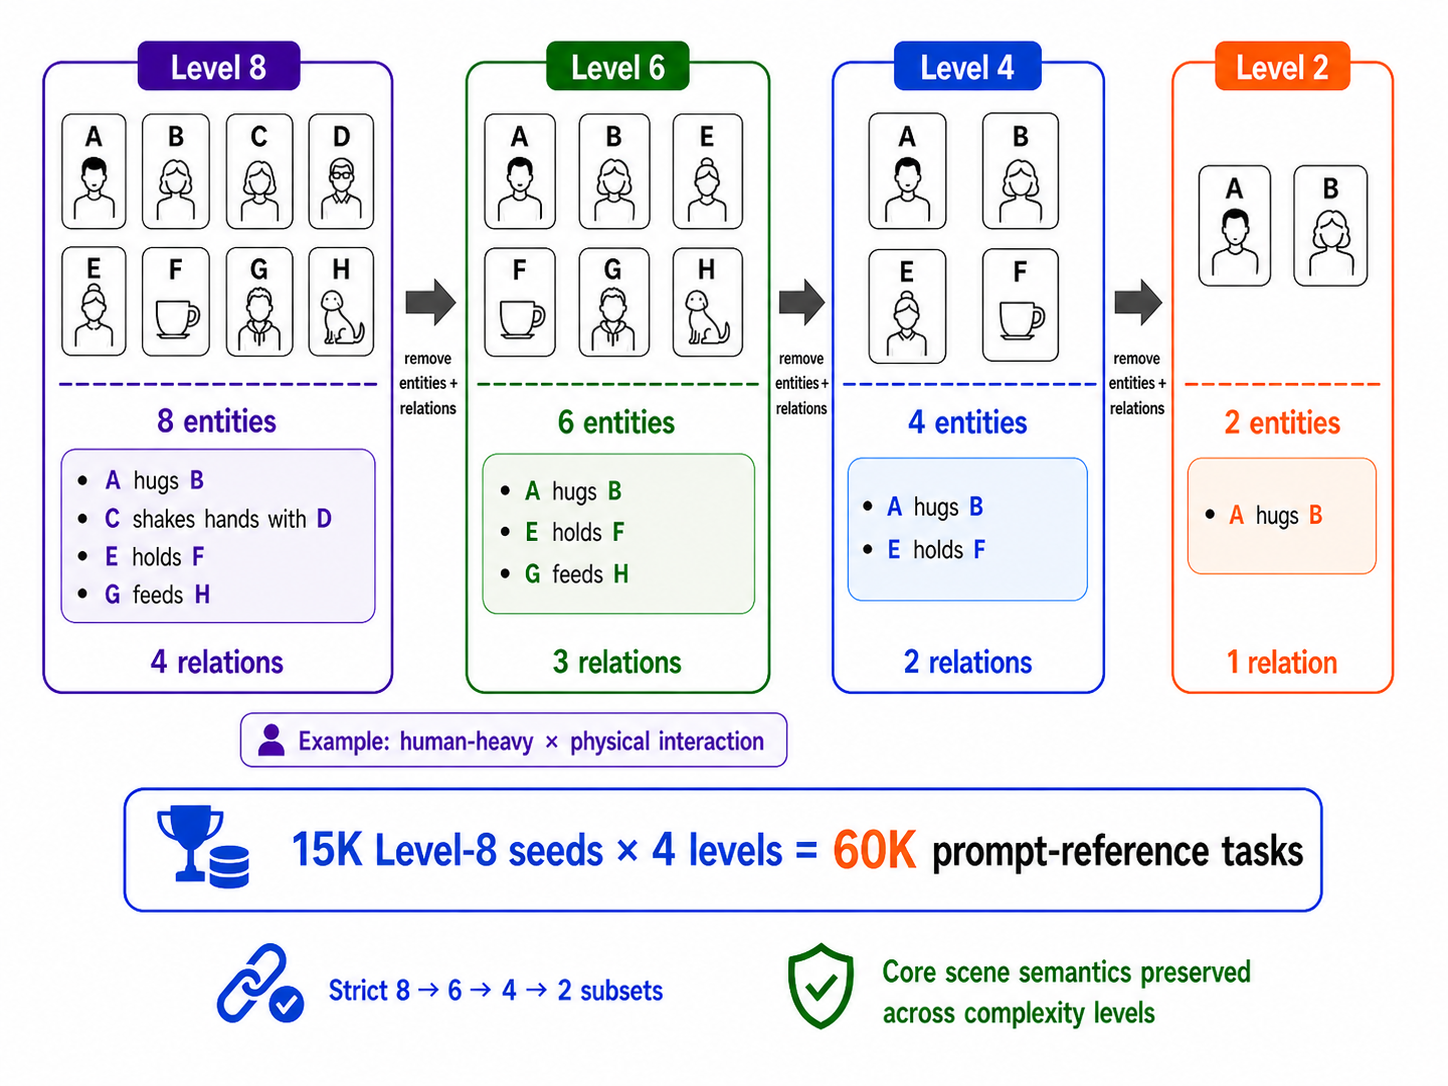
\includegraphics[width=0.5\textwidth,height=0.2\textheight]{hierarchical_prompt_construction.png}
    \caption{Hierarchical prompt construction. Each Level-8 seed is reduced into strict Level-6, Level-4, and Level-2 subsets by removing entities and their associated relations.}
    \label{fig:hierarchical_prompt_construction}
\end{figure*}


\begin{table}[t]
\centering
\small
\begin{tabular}{lcccc}
\toprule
\textbf{Ratio} & \textbf{L8} & \textbf{L6} & \textbf{L4} & \textbf{L2} \\
\midrule
Balanced     & 4H,4N & 3H,3N & 2H,2N & 1H,1N \\
Human-heavy  & 6H,2N & 4H,2N & 3H,1N & 2H,0N \\
Object-heavy & 2H,6N & 2H,4N & 1H,3N & 0H,2N \\
\bottomrule
\end{tabular}
\caption{Human/non-human composition for each ratio type and scene complexity level. H denotes human entities, and N denotes non-human entities.}
\label{tab:entity_ratio_levels}
\end{table}


We construct 60K prompt-reference tasks from 15K hierarchical seeds, where each seed produces four related prompts with $N \in \{8,6,4,2\}$ subjects. Each seed starts from an eight-subject scene and is reduced into six-, four-, and two-subject variants by removing entities and their associated relations. This hierarchical decomposition ensures that the core scene semantics remain invariant across complexity levels. Consequently, observed performance degradation can be more directly attributed to the increased density of entity-relation constraints rather than tangential shifts in prompt distribution.

The prompt space is factorized by subject count, human/object composition, and relation type, yielding $3 \times 3 \times 4 = 36$ buckets. Human/object composition includes balanced, human-heavy, and object-heavy configurations, with exact human/non-human counts specified in Table~\ref{tab:entity_ratio_levels}. Prompts are distributed approximately uniformly across the 36 buckets.

Relation type is organized into three broad categories: non-contact relations, occlusion relations, and physical interaction relations. We use separate template sets for the three categories to reduce boundary leakage during prompt generation. Non-contact relations include spatial or perceptual relations such as standing beside, facing, or looking at another subject. Occlusion relations describe partial visibility constraints without active engagement, such as one subject standing behind or partially blocking another subject. Physical interaction relations include both direct subject-to-subject interactions, such as hugging, petting, or shaking hands, and object-mediated interactions, such as holding or feeding.

Because relation types can overlap in natural scenes, we assign each task to the most restrictive applicable category, following the priority order: physical interaction $>$ occlusion $>$ non-contact. For each bucket, we also specify the participant structure of core relations, such as human-human, human-object, or object-object relations. Relations are assigned at the highest complexity level and then reduced together with the corresponding entities for lower-complexity prompts. To keep relation assignment interpretable, each entity participates in at most one core relation within a prompt.

All prompts are grounded in a white-studio setting with a global scale constraint. Specifically, each English prompt is prepended with: ``White studio. Keep all entities at realistic scale.'' This reduces background, lighting, layout, and unrealistic scale confounders, such as small objects being rendered at implausibly large sizes.

We apply automatic consistency checks using a rule-based parser and a lightweight LLM validator. These checks verify that assigned entities are explicitly mentioned, unassigned entities are excluded, human/non-human counts match the target bucket, lower-complexity prompts remain strict subsets of higher-complexity prompts, duplicate prompts are removed, the same entity is not reused as the subject of multiple independent relation statements, and interaction-specific keywords are not introduced into non-contact prompts.

\subsubsection{Reference Image Generation}

MIB uses a fixed pool of 80 reference subjects, including 30 human references and 50 non-human references. Human references cover diverse age groups, gender presentations, ethnicities, clothing styles, hairstyles, and visual appearances. Non-human references include animals, furniture, tools, wearable items, and common manipulable objects. This mixture allows MIB to evaluate both person-person binding and person-object or object-object binding under multi-subject personalized generation.

All reference images are generated using GPT-Image-1 and standardized as single-subject studio images at $512 \times 512$ resolution. Each reference image is produced as an isolated identity anchor, without multi-subject interactions or scene-specific relational context. The fixed reference pool allows the same subjects to be recombined across different prompts, making comparisons across complexity levels and relation types more controlled.

\subsubsection{Multi-subject Personalized Image Generation}

For each prompt-reference task, a personalized image generator receives a guiding prompt together with the corresponding reference images as visual conditioning inputs, and produces a candidate image. In our benchmark, reference subjects are provided as image-level identity anchors rather than as fine-tuned LoRA weights, ensuring a unified inference interface across generators. MIB constructs paired comparisons by placing two candidate generations under the same prompt-reference condition. This pairwise design controls for the prompt and reference set, so that annotators and evaluators compare only the relative quality of the two generated outputs.

For the Silver Set, we generate 60K candidate pairs using Nano Banana and MOSAIC. These two generators are selected because preliminary inspection shows complementary failure modes, including identity loss, subject omission, appearance leakage, and relation hallucination. This contrast creates informative pairwise supervision across existence, appearance, and interaction dimensions. Importantly, the reference images are generated separately using GPT-Image-1, so neither silver candidate generator is advantaged by sharing the same generation process as the reference pool. This separation reduces generator-specific leakage and makes the silver supervision less tied to the visual prior of either candidate generator.

For the Gold Set, we construct approximately 4K human-labeled candidate pairs. The Gold Set contains two subsets. First, for 1,260 main prompts, we generate candidate images using four state-of-the-art generators: GPT-Image-1.5, Flux2, Seedream 4.5, and GLM. For each prompt, we construct two pairwise comparisons: GPT-Image-1.5 versus Flux2, and Seedream 4.5 versus GLM, yielding 2,520 main-generator pairs. Rather than exhaustively comparing all six model pairs, we use two fixed cross-model matchups to balance comparison diversity and annotation cost. Second, we include 1,500 additional Nano Banana-versus-MOSAIC pairs to evaluate performance on seen-generator pairs under human annotation. For all Gold Set comparisons, both candidates are conditioned on the same reference images and guiding prompt, so the pairwise labels measure relative generation quality under an identical prompt-reference condition. Candidate order is randomized as Image A or Image B before annotation. Before labeling, we remove missing, corrupted, or blank generations through automatic validity checks.



\begin{table}[t]
\centering
\small
\renewcommand{\arraystretch}{1.25}
\setlength{\tabcolsep}{5pt}
\scalebox{0.95}{
\begin{tabular}{p{0.23\linewidth}p{0.33\linewidth}p{0.35\linewidth}}
\toprule
\textbf{Attribute} & \textbf{Silver Set} & \textbf{Gold Set} \\
\midrule
Purpose 
& MIE training 
& Human benchmark evaluation \\
\addlinespace[2pt]

Scale 
& 60,000 candidate pairs; 57,055 usable pairs 
& 4,020 human-labeled pairs \\
\addlinespace[2pt]

Prompt coverage 
& \multicolumn{2}{p{0.70\linewidth}}{Hierarchical prompts with strict high-to-low complexity subsets, approximately uniformly distributed across relation type, human/object ratio, and subject count.} \\
\addlinespace[2pt]

Candidate generators 
& Nano Banana, MOSAIC 
& GPT-Image-1.5, Flux2, Seedream 4.5, GLM; plus Nano Banana/MOSAIC for seen-generator evaluation \\
\addlinespace[2pt]

Annotation source 
& SOP-guided dual VLM consensus 
& Double-blind human annotation \\
\addlinespace[2pt]

Annotators 
& Gemini-2.5-Flash and Gemini-3.1-Flash-Lite 
& Two independent human annotators per pair \\
\addlinespace[2pt]

Label types 
& Pairwise preference; Existence; Appearance; Interaction 
& Pairwise preference; Existence; Appearance; Interaction \\
\addlinespace[2pt]

Evaluation role 
& Train 51K / Val 2.8K / Test 2.9K 
& Seen-generator: 1,500 pairs; unseen-generator: 2,520 pairs \\
\bottomrule
\addlinespace[3pt]
\end{tabular}
}
\caption{Dataset statistics for MIB. The Silver Set provides scalable SOP-guided VLM supervision for training MIE, while the Gold Set is fully human-labeled under a double-blind protocol.}
\label{tab:dataset_statistics}
\end{table}


\subsubsection{Label Construction}
\label{sec:method_label}
MIB provides two complementary forms of supervision: pairwise preference labels for global ranking and diagnostic labels for failure localization. Pairwise preference captures which candidate is better overall under the same prompt-reference condition, while diagnostic labels identify whether each candidate fails in subject existence, reference appearance preservation, or interaction grounding.

\paragraph{Pairwise preference.}
Rather than assigning absolute scores to individual images, we adopt pairwise preference as the primary global ranking signal. Given two generated images $A$ and $B$ produced under the same prompt and reference set, the annotator determines which image is the better overall result, without assigning a numerical score to either candidate in isolation.

This design is motivated by two considerations. First, absolute scoring in multi-subject personalized generation is difficult to calibrate: the failure space is heterogeneous, and different annotators may apply inconsistent severity scales when mapping compositional defects to scalar values. Pairwise judgment reduces this calibration burden by asking for a relative comparison under a shared prompt-reference condition. Second, pairwise preference captures graded severity information that categorical labels alone cannot represent. Two images may exhibit the same type of failure yet differ substantially in degree; the preference signal resolves this ambiguity by indicating which failure is more tolerable.

\paragraph{Diagnostic labels.}
While pairwise preference captures overall quality ranking, it does not localize where or why a generated image fails. We therefore decompose multi-subject generation quality into three complementary diagnostic dimensions:
\begin{itemize}
    \item \textbf{Existence}: whether all requested reference subjects are present without omission, duplication, or severe unidentifiable collapse.
    \item \textbf{Appearance}: whether the generated image preserves the physical structure and local appearance of the requested reference subjects, without severe distortion or cross-subject feature bleeding.
    \item \textbf{Interaction}: whether subject-to-subject relations, actions, and object assignments are aligned with the prompt.
\end{itemize}

For diagnostic labels, we adopt a soft aggregation strategy. In cases of annotator disagreement, the final dimension score is computed as the average of the two annotations. For example, if annotator A assigns scores $(1, 1, 0)$ and annotator B assigns $(1, 0, 0)$ across Existence, Appearance, and Interaction, respectively, the resolved label is $(1, 0.5, 0)$. This treatment reflects the different roles of the two label types: the pairwise winner must be unambiguous to serve as a reliable ranking target, whereas fractional diagnostic scores encode annotator uncertainty and provide softer supervision for evaluator training and analysis.

\paragraph{MIB-Silver annotation with SOP-guided VLM judges.}
Training MIE requires large-scale pairwise preference and diagnostic supervision. However, manually annotating 60K image pairs is prohibitively slow and expensive given the multi-dimensional verification required for multi-subject personalized generation. We therefore construct MIB-Silver using SOP-guided frontier VLM judges, while reserving human annotations exclusively for MIB-Gold.

To align scalable machine annotation with the intended human evaluation protocol, we use a unified Standard Operating Procedure (SOP) for both VLM and human annotators. The SOP decomposes each comparison into a three-stage verification process: 1) \emph{Existence}, verifying the physical presence of all referenced subjects; 2) \emph{Appearance}, checking structural integrity and identity or appearance fidelity against the references; and 3) \emph{Interaction}, assessing whether spatial relations, physical interactions, and object assignments follow the prompt.

Unlike generic preference prompting, which can collapse into uninterpretable holistic judgments or over-weight global aesthetics, our SOP requires the judge to produce candidate-specific flaw logs before rendering a final preference decision. This errors-first structure encourages the judge to ground its decision in concrete compositional failures, such as missing entities, identity swaps, appearance leakage, and interaction violations.

To further improve label precision and mitigate model-specific annotation bias, we use a cross-model consensus mechanism. We independently query two frontier VLMs, \texttt{gemini-2.5-flash} and \texttt{gemini-3.1-flash-lite-preview}, using the identical SOP. We retain only the comparisons for which both models produce the same pairwise preference. Although this intersection rule reduces total yield, it acts as a conservative precision filter by pruning examples where preference may be driven by ambiguous image quality or idiosyncratic model behavior. The resulting high-agreement subset serves as scalable training supervision for MIE, and its effectiveness is validated against the human-annotated Gold Set. The exact SOP prompt is reproduced in Appendix~\ref{sec:app_SOP}.

\paragraph{MIB-Gold annotation with double-blind human evaluation.}
MIB-Gold labels are collected exclusively from human annotators under a double-blind protocol. Each of the approximately 4K Gold Set pairs described above is independently reviewed by two annotators, who provide both a pairwise preference label and diagnostic labels for Existence, Appearance, and Interaction. We require strict consensus for preference labels, discarding pairs with annotator disagreement, while diagnostic disagreements are averaged to produce soft labels.

\paragraph{Annotation agreement.}
To quantify annotation reliability, we measure agreement separately for Silver VLM annotations and Gold human annotations. As shown in Table~\ref{tab:annotation_agreement}, global preference labels achieve high agreement in both settings, while diagnostic labels are less consistent, especially for appearance and interaction. This supports our design choice of using strict consensus for pairwise preference and soft aggregation for diagnostic supervision.

\begin{table}[t]
\centering
\small
\renewcommand{\arraystretch}{1.15}
\begin{tabular}{lcc}
\toprule
\textbf{Dimension} & \textbf{Silver VLM Agreement} & \textbf{Gold Human Agreement} \\
\midrule
Preference  & 95.1\% & 91.8\% \\
Existence   & 89.1\% & 92.5\% \\
Appearance  & 69.0\% & 80.2\% \\
Interaction & 71.9\% & 74.8\% \\
\bottomrule
\end{tabular}
\caption{Annotation agreement by evaluation dimension. Preference labels exhibit high agreement for both Silver VLM annotation and Gold human annotation, while fine-grained diagnostic dimensions show lower agreement, motivating strict consensus for preference labels and soft aggregation for diagnostic labels.}
\label{tab:annotation_agreement}

\end{table}



\subsection{Evaluator Modeling}

The primary goal of MIBE is to establish a rigorous evaluation framework for multi-subject personalized image generation. To demonstrate that this framework is not only descriptive but also operationally useful, we instantiate a learned evaluator, termed \textbf{Multi-subject Interaction Evaluator (MIE)}, as a proof-of-concept metric trained on MIB-Silver and assessed on MIB-Gold. Importantly, MIE is not intended to be the sole contribution of this work. Rather, it serves as the first benchmark-enabled evaluator built from MIBE, validating that the structured supervision provided by our benchmark can be translated into an automatic metric that better reflects human judgment in this challenging regime.

\paragraph{Motivation.}
As discussed in the previous sections, the central difficulty of multi-subject personalized image generation is not merely global realism or coarse text-image alignment, but \emph{binding}: the evaluator must determine whether each generated subject faithfully corresponds to the intended reference identity, whether local appearance is preserved without cross-subject leakage, and whether the specified interactions are assigned to the correct entities. Existing metrics typically capture only fragments of this problem. Text-image metrics often reward overall semantic plausibility without checking identity fidelity, while reference-image similarity metrics can capture local resemblance yet ignore prompt-conditioned role assignment and interaction structure. This motivates an evaluator that jointly reasons over the \emph{prompt}, the \emph{reference set}, and the \emph{generated candidate image}.

\paragraph{Input-Output Formulation.}
For each task, let $p$ denote the prompt, $R=\{r_1,\dots,r_N\}$ denote the set of reference images, and let $y$ denote a candidate generation. MIE is a reference-conditioned multimodal evaluator that maps the triplet $(R,p,y)$ to two types of outputs:
\begin{enumerate}
    \item a scalar quality score $s_\theta(R,p,y)\in\mathbb{R}$ used for global pairwise ranking, and
    \item a three-dimensional diagnostic prediction vector
    \[
    \hat d_\theta(R,p,y) = (\hat d_{\text{exist}}, \hat d_{\text{app}}, \hat d_{\text{inter}}),
    \]
    corresponding to \emph{Existence}, \emph{Appearance}, and \emph{Interaction}.
\end{enumerate}

The scalar score provides a continuous global signal that can distinguish mild degradation from catastrophic collapse, while the diagnostic outputs provide interpretable image-level attribution over the dominant failure modes in multi-subject generation.

\paragraph{Pairwise Comparison Setup.}
Our evaluator follows the same pairwise protocol used in both MIB-Silver and MIB-Gold. For a task with two candidate images $(y^A, y^B)$ generated under the same prompt-reference condition, MIE processes the two candidates independently but under the same conditioning context $(R,p)$. This produces two scalar scores,
\[
s^A = s_\theta(R,p,y^A), \qquad s^B = s_\theta(R,p,y^B),
\]
and two diagnostic predictions,
\[
\hat d^A = \hat d_\theta(R,p,y^A), \qquad \hat d^B = \hat d_\theta(R,p,y^B).
\]
The preferred image is then induced by the score difference:
\[
y^A \succ y^B \quad \text{iff} \quad s^A > s^B.
\]
This design mirrors the annotation procedure directly: annotators compare two candidate generations under an identical prompt-reference condition, while our model learns to assign each candidate an absolute latent utility score whose difference explains the pairwise preference.

\paragraph{Architecture.}
We implement MIE as a lightweight vision-language evaluator with a shared multimodal backbone and two task-specific heads. The multimodal input consists of the full reference set, the candidate image, and the textual prompt. Rather than encoding only the generated image or only the references, the model jointly encodes the entire evaluation context, allowing it to reason over identity fidelity, subject correspondence, and interaction semantics in a unified representation space.

Given the final hidden representation produced by the backbone, MIE extracts a global contextual feature and feeds it into two trainable heads:
\begin{itemize}
    \item a \textbf{ranking head}, which outputs the scalar score $s_\theta(R,p,y)$, and
    \item a \textbf{diagnostic head}, which outputs three logits corresponding to Existence, Appearance, and Interaction.
\end{itemize}

This dual-head design reflects the dual role of evaluation in our setting. The ranking head answers the question \emph{which image is better overall}, while the diagnostic head answers \emph{why} a particular image fails. By coupling the two, MIE preserves both ranking separability and interpretability.

\paragraph{Why Ranking and Diagnosis Must Be Learned Jointly.}
A purely diagnostic evaluator is insufficient for multi-subject personalized generation. In particular, binary error labels alone cannot capture failure severity. For example, an image missing one subject and another image missing several subjects may both receive Existence$=0$, even though human annotators consistently prefer the less severely collapsed candidate. Pairwise preference therefore acts as the channel through which relative severity becomes learnable.

Conversely, a purely scalar reward model is also unsatisfactory. A single global score can correlate with human preference without revealing whether the failure arose from omission, appearance corruption, or incorrect interaction binding. Such black-box behavior weakens interpretability and limits the evaluator's usefulness for diagnosis and model development. MIE addresses this by jointly learning a continuous ranking signal and structured diagnostic predictions. In this formulation, pairwise preference captures \emph{how bad} a generation is overall, while the three dimensions reveal \emph{what kind} of failure is present.

\paragraph{Training Objective.}
MIE is trained exclusively on MIB-Silver, where each pair provides a preference label together with image-level diagnostic annotations for both candidates. Let $w \in \{+1,-1\}$ denote the pairwise preference target, where $w=+1$ indicates that candidate $A$ is preferred to candidate $B$, and $w=-1$ indicates the reverse. We optimize a margin-based ranking loss:
\[
\mathcal{L}_{\text{rank}}
=
\max\bigl(0, m - w(s^A - s^B)\bigr),
\]
where $m>0$ is the ranking margin. This objective encourages the preferred image to receive a higher score than the dispreferred image by at least a fixed margin, thereby improving ranking separability.

In addition to pairwise preference, each candidate image is supervised by a three-dimensional diagnostic target. Let $d^A,d^B \in [0,1]^3$ denote the diagnostic labels for candidates $A$ and $B$, respectively. We optimize an image-level diagnostic loss on both candidates:
\[
\mathcal{L}_{\text{diag}}
=
\frac{1}{2}
\left[
\ell_{\text{diag}}(\hat d^A, d^A) + \ell_{\text{diag}}(\hat d^B, d^B)
\right],
\]
where $\ell_{\text{diag}}$ is a per-dimension binary supervision loss. The final training objective is
\[
\mathcal{L}
=
\alpha \mathcal{L}_{\text{rank}} + \beta \mathcal{L}_{\text{diag}},
\]
where $\alpha$ and $\beta$ balance global ranking and structured diagnosis.

This objective closely matches the benchmark design. The pairwise term preserves the main human decision signal, while the image-level term injects fine-grained structure into the evaluator, preventing it from collapsing into an opaque preference model that ignores the specific failure dimensions emphasized by our benchmark.

\paragraph{Training Regime.}
To ensure that the evaluator remains practical rather than overly specialized, we adopt a lightweight fine-tuning strategy over a pretrained vision-language backbone. We explore parameter-efficient and partial-tuning variants, including head-only adaptation, selective backbone layer tuning, and LoRA-style updates. This design choice is intentional: our goal is not to maximize performance through brute-force scaling, but to test whether the supervision enabled by MIBE is itself sufficiently informative to train a deployable evaluator with strong human alignment.

\paragraph{Role Within MIBE.}
We emphasize that MIE should be interpreted as a \emph{benchmark-enabled evaluator baseline} rather than the sole endpoint of this work. The broader claim of MIBE is that once multi-subject personalization failures are operationalized through a high-quality human gold benchmark and a large-scale silver supervision resource, it becomes possible to train automatic evaluators that preserve ranking separability, expose interpretable failure modes, and generalize across generators more faithfully than existing metrics. In this sense, MIE serves as a concrete demonstration of the utility of MIBE: the benchmark does not merely measure failure, but also enables the development of better evaluators for this previously under-served setting.








\section{Results}
\subsection{MIB Label Alignment Results}
\subsubsection{MIB-Silver Results}

When constructing the MIB-Silver dataset label, we apply the SOP detailed in Section~\ref{sec:method_label} across a large-scale corpus of $\sim$60K candidate pairs, which also yields compelling insights into VLM evaluation behavior. Notably, the two VLM judges achieve a robust \emph{Preference Agreement} of $95.1\%$ ($56,909 / 59,852$ valid overlapping tasks). Looking at the fundamental sub-scores (Figure~\ref{fig:agreement_analysis}a), the models exhibit high consensus on \emph{Existence} ($89.1\%$) and substantial agreement on \emph{Interaction} ($71.9\%$) and \emph{Appearance} ($69.0\%$). This overall high preference consensus demonstrates that the SOP effectively anchors the models' global decision-making, confirming that the intersection-filtered labels are highly reliable and well-suited for training our lightweight evaluator. 

\begin{figure}[t]
    \centering
    \begin{subfigure}[b]{0.32\textwidth}
        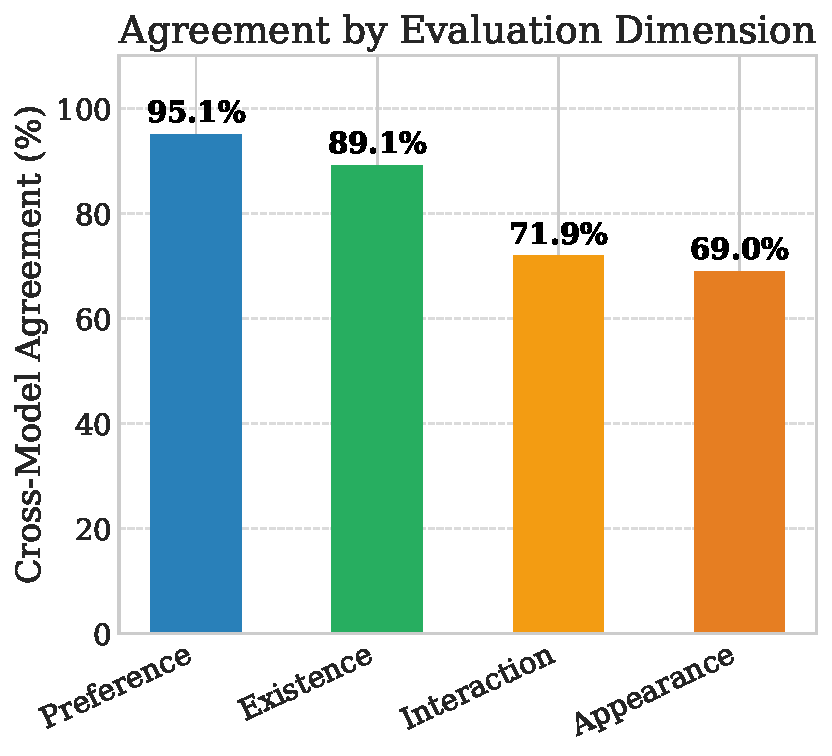
\includegraphics[width=\textwidth]{figures/overall_agreement.pdf}
        \caption{By Evaluation Dimension}
        \label{fig:agree_dim}
    \end{subfigure}
    \hfill
    \begin{subfigure}[b]{0.32\textwidth}
        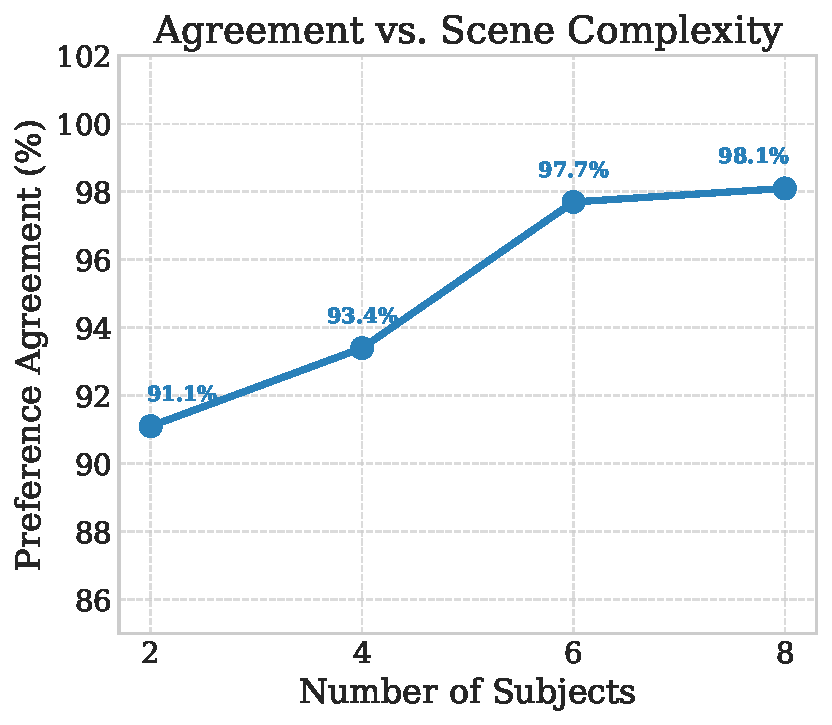
\includegraphics[width=\textwidth]{figures/agreement_by_subject.pdf}
        \caption{By Subject Count}
        \label{fig:agree_subj}
    \end{subfigure}
    \hfill
    \begin{subfigure}[b]{0.32\textwidth}
        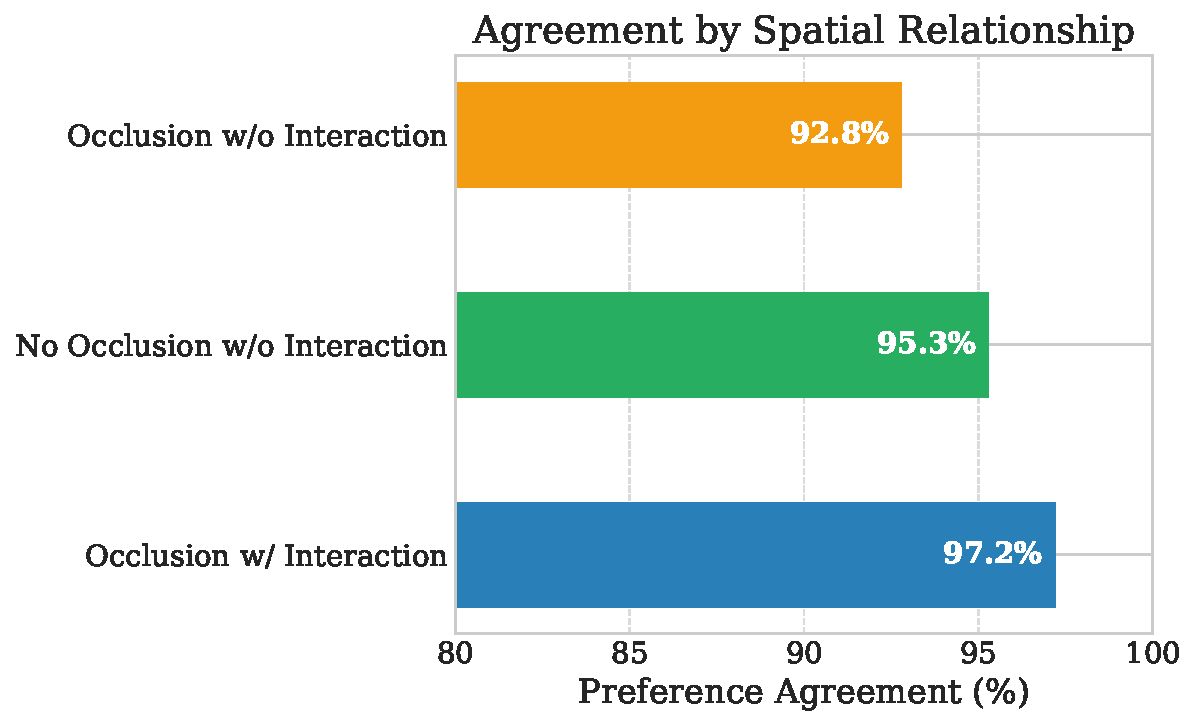
\includegraphics[width=\textwidth]{figures/agreement_by_tag.pdf}
        \caption{By Spatial Relationship}
        \label{fig:agree_tag}
    \end{subfigure}
    \caption{Cross-model agreement analysis on 60K tasks between \texttt{gemini-2.5-flash} and \texttt{gemini-3.1-flash-lite-preview}. (a) Models reliably converge on global preference but exhibit higher variance on fine-grained appearance. (b) Counter-intuitively, preference agreement increases with the number of subjects, as catastrophic compositional failures in dense scenes make the ``less collapsed'' image trivially obvious. (c) Explicitly prompted interactions provide stronger contextual grounding, yielding the highest agreement.}
    \label{fig:agreement_analysis}
\end{figure}

\paragraph{Qualitative Analysis of SOP Effectiveness.}
To further validate the robustness of our SOP, we qualitatively examine cases where both \texttt{gemini-2.5-flash} and \texttt{gemini-3.1-flash-lite-preview} reach a strict consensus on all sub-scores and the final preference (Figure~\ref{fig:sop_demos}). The externalized \emph{flaw logs} reveal that the VLMs successfully internalize the multi-dimensional constraints defined in the SOP. This is initially evident in the models' ability to enforce precise semantic adherence for action and target grounding. For instance, in Figure~\ref{fig:sop_demos}(a), the VLMs correctly penalize Candidate B for hallucinating an interaction target (using a stick instead of a hand) and missing a secondary interaction entirely. Beyond semantic accuracy, the SOP effectively drives strict geometric and physical verification. As highlighted in Figure~\ref{fig:sop_demos}(b) and (d), the models identify violations of realistic physics, such as a floating mug embedded in a strange artifact, and catch severe scale distortions like an abnormally giant fried chicken. Furthermore, the evaluators demonstrate a keen sensitivity to fine-grained attribute fidelity. As seen in Figure~\ref{fig:sop_demos}(c) and (d), they effectively scrutinize wardrobe and identity details, successfully catching subtle errors like an incorrect donut color (pink instead of chocolate) or a wrong suitcase color (black instead of white). Importantly, this diagnostic rigor remains robust even in highly complex scenes. Figure~\ref{fig:sop_demos}(e) demonstrates a dense 6-subject composition where Candidate B suffers from severe collapse; despite the visual clutter, both models accurately and consistently isolate multiple concurrent failures across appearance (wrong clothing) and interactions (missing petting, closing, and carrying actions).

Overall, these qualitative results confirm that the ``errors-first'' scaffolding successfully prevents the VLMs from falling back on holistic aesthetic biases, forcing them to conduct rigorous, localized compositional verification.

\subsubsection{MIB-Gold Results}

While Section~4.1.1 shows that our SOP yields reliable large-scale silver supervision, \texttt{MIB-Gold} serves a different role: it is the human-controlled benchmark that tests whether multi-subject evaluation remains reliable once ambiguity is no longer filtered by model-model agreement alone. In total, \texttt{MIB-Gold} contains 4,020 raw pair groups. Of these, 1,500 come from the \texttt{Nano Banana + Mosaic} subset, while the remaining 2,520 are drawn from a broader cross-platform pool. After preference-consistency filtering, the retained-pair rate is 94.1\% for the \texttt{Nano Banana + Mosaic} subset and 90.4\% for the broader cross-platform subset, indicating that difficulty is not uniform across generator sources.

This difficulty is structured rather than noisy. As shown in Figure~\ref{fig:mib_gold_benchmark}, human preference consistency rises from 87.0\% at level 2 to 94.9\% at level 6, and remains high at level 8. Even as scenes become denser and compositionally more demanding, annotators still converge on a stable preference signal after consistency control. Thus, \texttt{MIB-Gold} does not simply introduce additional annotation variance; it reveals a meaningful difficulty distribution while preserving a dependable human judgment target.

Taken together, these results establish \texttt{MIB-Gold} as more than a small human-labeled subset. It is the benchmark layer that makes the rest of our evaluation possible: difficult enough to expose non-trivial disagreement, yet reliable enough to serve as the reference set for testing both existing metrics and learned evaluators.

\begin{figure}[t]
    \centering
    
\includegraphics[width=\linewidth]{figures/section_4_1_2_gold_benchmark.png}
    \caption{Human annotation findings on `MIB-Gold`. Left: preference consistency by benchmark level. Right: preference consistency by spatial relationship. The lower retention in the broader cross-platform subset indicates that `MIB-Gold` captures a meaningful benchmark difficulty gap rather than annotation noise.}
    \label{fig:mib_gold_benchmark}
\end{figure}


\subsection{Evaluator Results on MIB-Gold}
\subsubsection{Existing Metrics Fail on MIB-Gold}

To establish a comprehensive performance ceiling and evaluate the limitations of existing metrics in multi-subject scenarios, we select a representative suite of baselines spanning four distinct paradigms: 

(1) \textbf{Low-level Reconstruction Metrics}: PSNR~\cite{hore2010image}, SSIM~\cite{wang2004image}, and MS-SSIM~\cite{wang2003multiscale} are included to measure pixel-level fidelity; 

(2) \textbf{Semantic Alignment Metrics}: DINOv2~\cite{oquab2023dinov2}, CLIP~\cite{radford2021learning}, and SigLIP~\cite{zhai2023sigmoid} (both Text-based and Image-based) are used to evaluate high-level semantic consistency and identity similarity; 

(3) \textbf{General Human Preference Models}: PickScore~\cite{kirstain2023pick}, ImageReward~\cite{xu2023imagereward}, and HPS v2.1~\cite{wu2023human}, which are specifically trained on human feedback for text-to-image alignment and aesthetics; 

(4) \textbf{Identity-Specific Metrics}: SCR (Subject Consistency Rate)~\cite{chen2026identities}, which focus on  identity-preserving features critical for personalization.

By evaluating this broad spectrum, we aim to test whether current automated metrics, often designed for single-subject or generic scenes, can effectively handle the ``binding" challenges, such as identity swapping and complex interactions, present in our benchmark.

% Table~\ref{tab:overall_metrics} summarizes the mean score of each model on the benchmark. For similarity-style metrics such as PSNR, SSIM, MS-SSIM, DINO, CLIP-T, CLIP-I, SigLIP-T, SigLIP-I, ImageReward, PickScore, and HPS v2.1, larger values indicate better performance. For SCR, smaller values are preferable.

% \begin{table}[t]
% \centering
% \scriptsize
% \setlength{\tabcolsep}{6pt}
% \caption{Overall mean score of each model.}
% \label{tab:overall_metrics}
% \begin{tabular}{lcccc}
% \hline
% \textbf{Metric} & \textbf{GLM} & \textbf{FLUX-2} & \textbf{GPT-image-1.5-high} & \textbf{Seedream-4.5} \\
% \hline
% PSNR & 9.2313 & \textbf{11.0662} & 10.4655 & 9.3190 \\
% SSIM & 0.6308 & 0.7195 & 0.7159 & \textbf{0.7354} \\
% MS-SSIM & 0.5412 & 0.6215 & 0.5983 & \textbf{0.6358} \\
% DINOv2 & 0.5410 & 0.6300 & 0.6627 & \textbf{0.6384} \\
% CLIP-T & 0.3430 & 0.3569 & 0.3564 & \textbf{0.3599} \\
% CLIP-I & 0.7144 & 0.7388 & \textbf{0.7488 }& 0.7356 \\
% SigLIP-T & 0.1809 & \textbf{0.2084} & 0.2050 & 0.2036 \\
% SigLIP-I & 0.7235 & 0.7379 & \textbf{0.7526} & 0.7453 \\
% PickScore & 20.7658 &\textbf{ 21.2998 }& 20.8713 & 21.1139 \\
% ImageReward & 0.7122 & 1.1499 & 1.0351 & \textbf{1.1638} \\
% HPS v2.1 & 0.2827 & 0.2970 & 0.2826 & \textbf{0.2979} \\
% \hline 
% SCR & 0.2006 & 0.2003 & \textbf{0.1245} & 0.1436 \\
% \hline
% \end{tabular}
% \end{table}

 We compare automatic metrics against human pairwise preference annotations. After excluding 49 samples marked as prompt-ilogical, the analysis uses 4,991 valid pairwise comparisons. For each comparison, we determine which model is preferred by the annotator and then check whether each automatic metric would rank the same model higher on the corresponding sample. In Figure~\ref{fig:metric_agreement_subject_count}, we report pairwise agreement with human preference, where 0.5 corresponds to random guessing in a balanced binary comparison.

% \begin{figure}[t]
% \centering
% 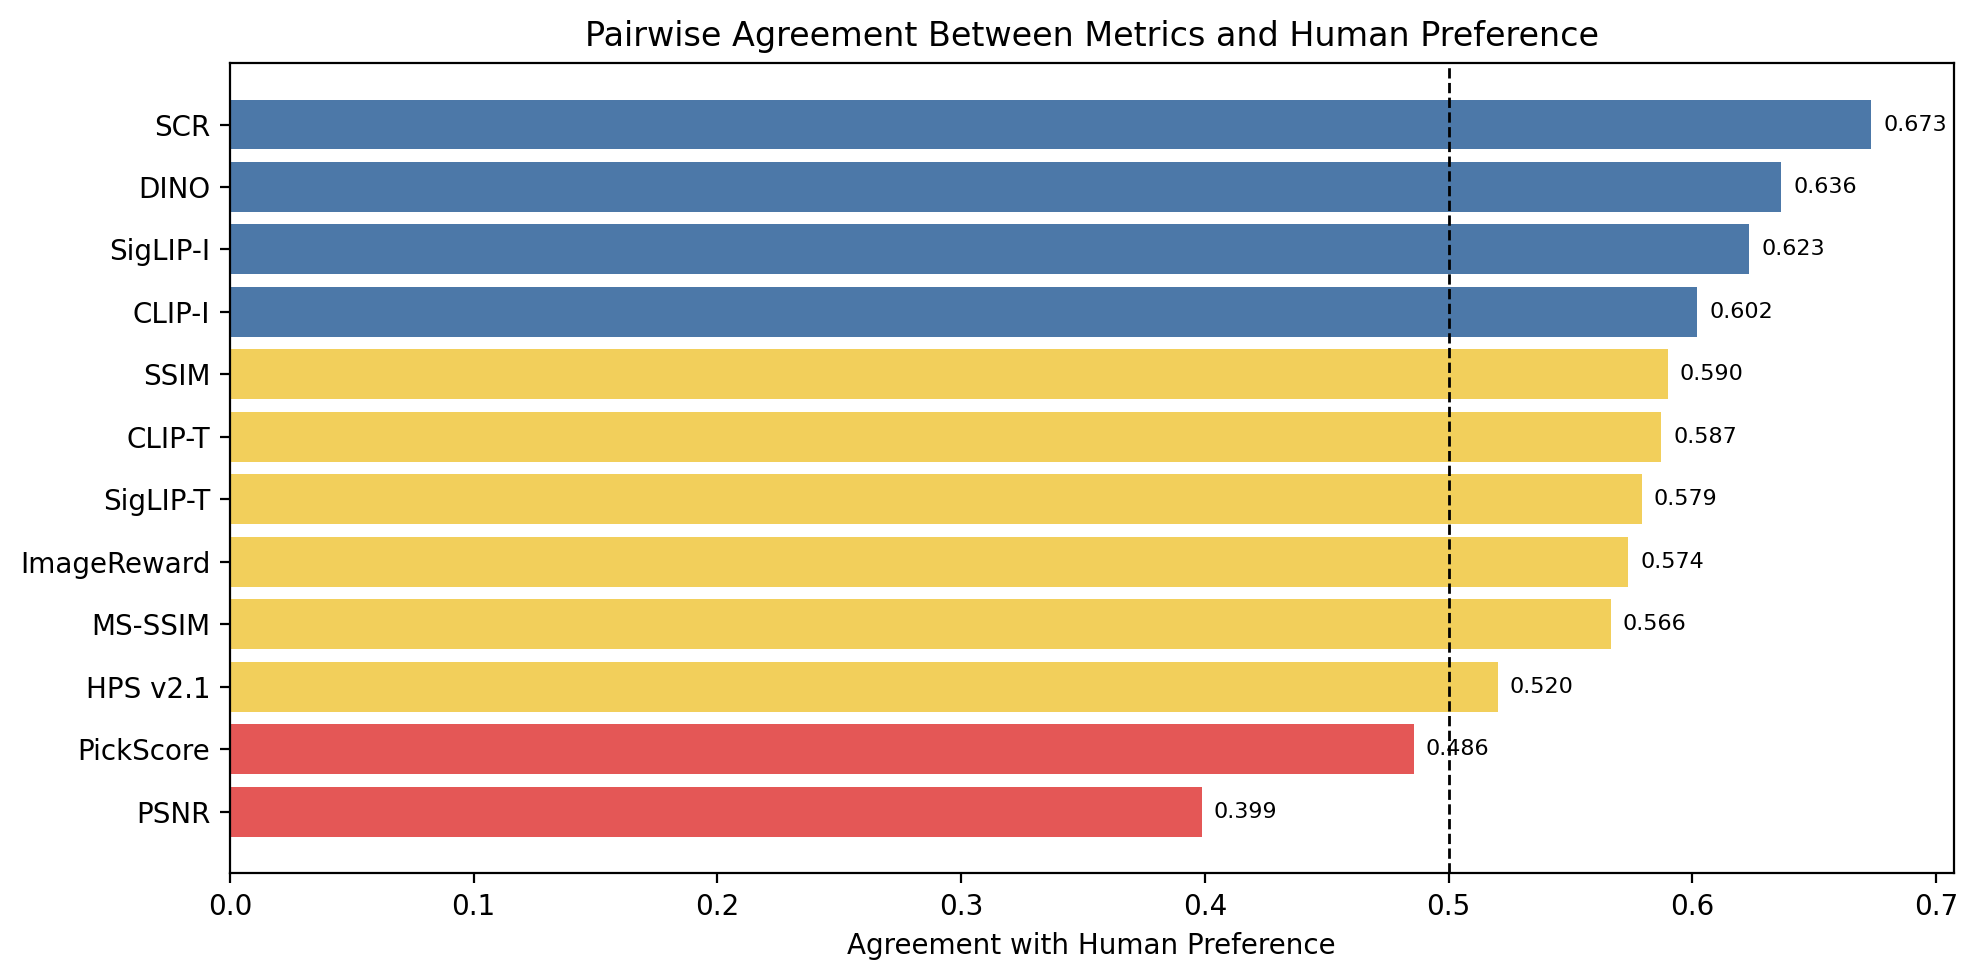
\includegraphics[width=\linewidth]{figures/human_vs_metric_pairwise_accuracy.png}
% \caption{Pairwise agreement between automatic metrics and human preference. The dashed line indicates random-choice accuracy (0.5).}
% \label{fig:human_metric_pairwise_accuracy}
% \end{figure}


The comparison shows that the automatic baselines are far from uniformly reliable as proxies for human preference. Several metrics remain only slightly above random choice, including HPS v2.1 (0.5201), while PickScore (0.4857) falls slightly below the random baseline and PSNR (0.3987) is substantially misaligned with human judgments in this setting. Therefore, these metrics should not be treated as dependable replacements for direct human evaluation on this benchmark.

At the same time, the results are not uniformly negative across all baselines. Though metrics like SCR, DINOv2, and SigLIP-I show non-trivial alignment, these successes are largely confined to single-dimensional facets such as identity preservation or global semantic consistency. The failure of general-purpose preference scorers (e.g., PickScore, HPS v2.1) to significantly outperform random choice, coupled with the high variance across different metric categories, reveals a fundamental gap in current evaluation paradigms. These fragmented baselines lack a unified reasoning framework to handle the complex ``binding" problem (existence, identity, and interaction) inherent in human judgment. This misalignment underscores the critical need for a more structured, multi-dimensional evaluator that can faithfully replicate the human decision-making process.

\subsubsection{MIE Aligns Better with Human Preference}

If Section~4.2.1 establishes that existing metrics are fundamentally misaligned with human preference on \texttt{MIB-Gold}, the next question is whether this benchmark can be used to train a better evaluator. Our results show that it can. Across all six exported checkpoints, the strongest variant is \texttt{qwen35\_4b\_lora\_layer}, which achieves an overall pairwise accuracy of 0.922, including 0.982 on the seen-generator subset and 0.884 on the unseen-generator subset. This substantially exceeds the strongest third-party baseline, showing that supervision derived from \texttt{MIB} can be translated into a materially stronger human-aligned metric.

The gains are not limited to pairwise ranking. The same 4B LoRA-layer model reaches a macro-F1 of 0.818, indicating that the evaluator is not merely learning a shallow preference score, but capturing a meaningful portion of the fine-grained diagnostic structure underlying human judgments. This matters because the binding problem in multi-subject personalization is inherently multi-dimensional: a useful evaluator must jointly reason about existence, appearance, and interaction rather than collapse everything into a single weak aesthetic signal.

More broadly, the six-checkpoint comparison now supports a full scaling narrative. LoRA-layer variants consistently outperform their layer-only counterparts, and the largest LoRA-based model achieves the strongest overall human alignment. As shown in Figure~\ref{fig:mie_alignment}, the advantage is visible not only in pairwise accuracy but also in the category-level F1 breakdown. Thus, \texttt{MIB} does not only expose the failure of existing metrics; it also enables the training of a new evaluator that tracks human preference far more faithfully in multi-subject settings.

\begin{figure}[t]
    \centering
    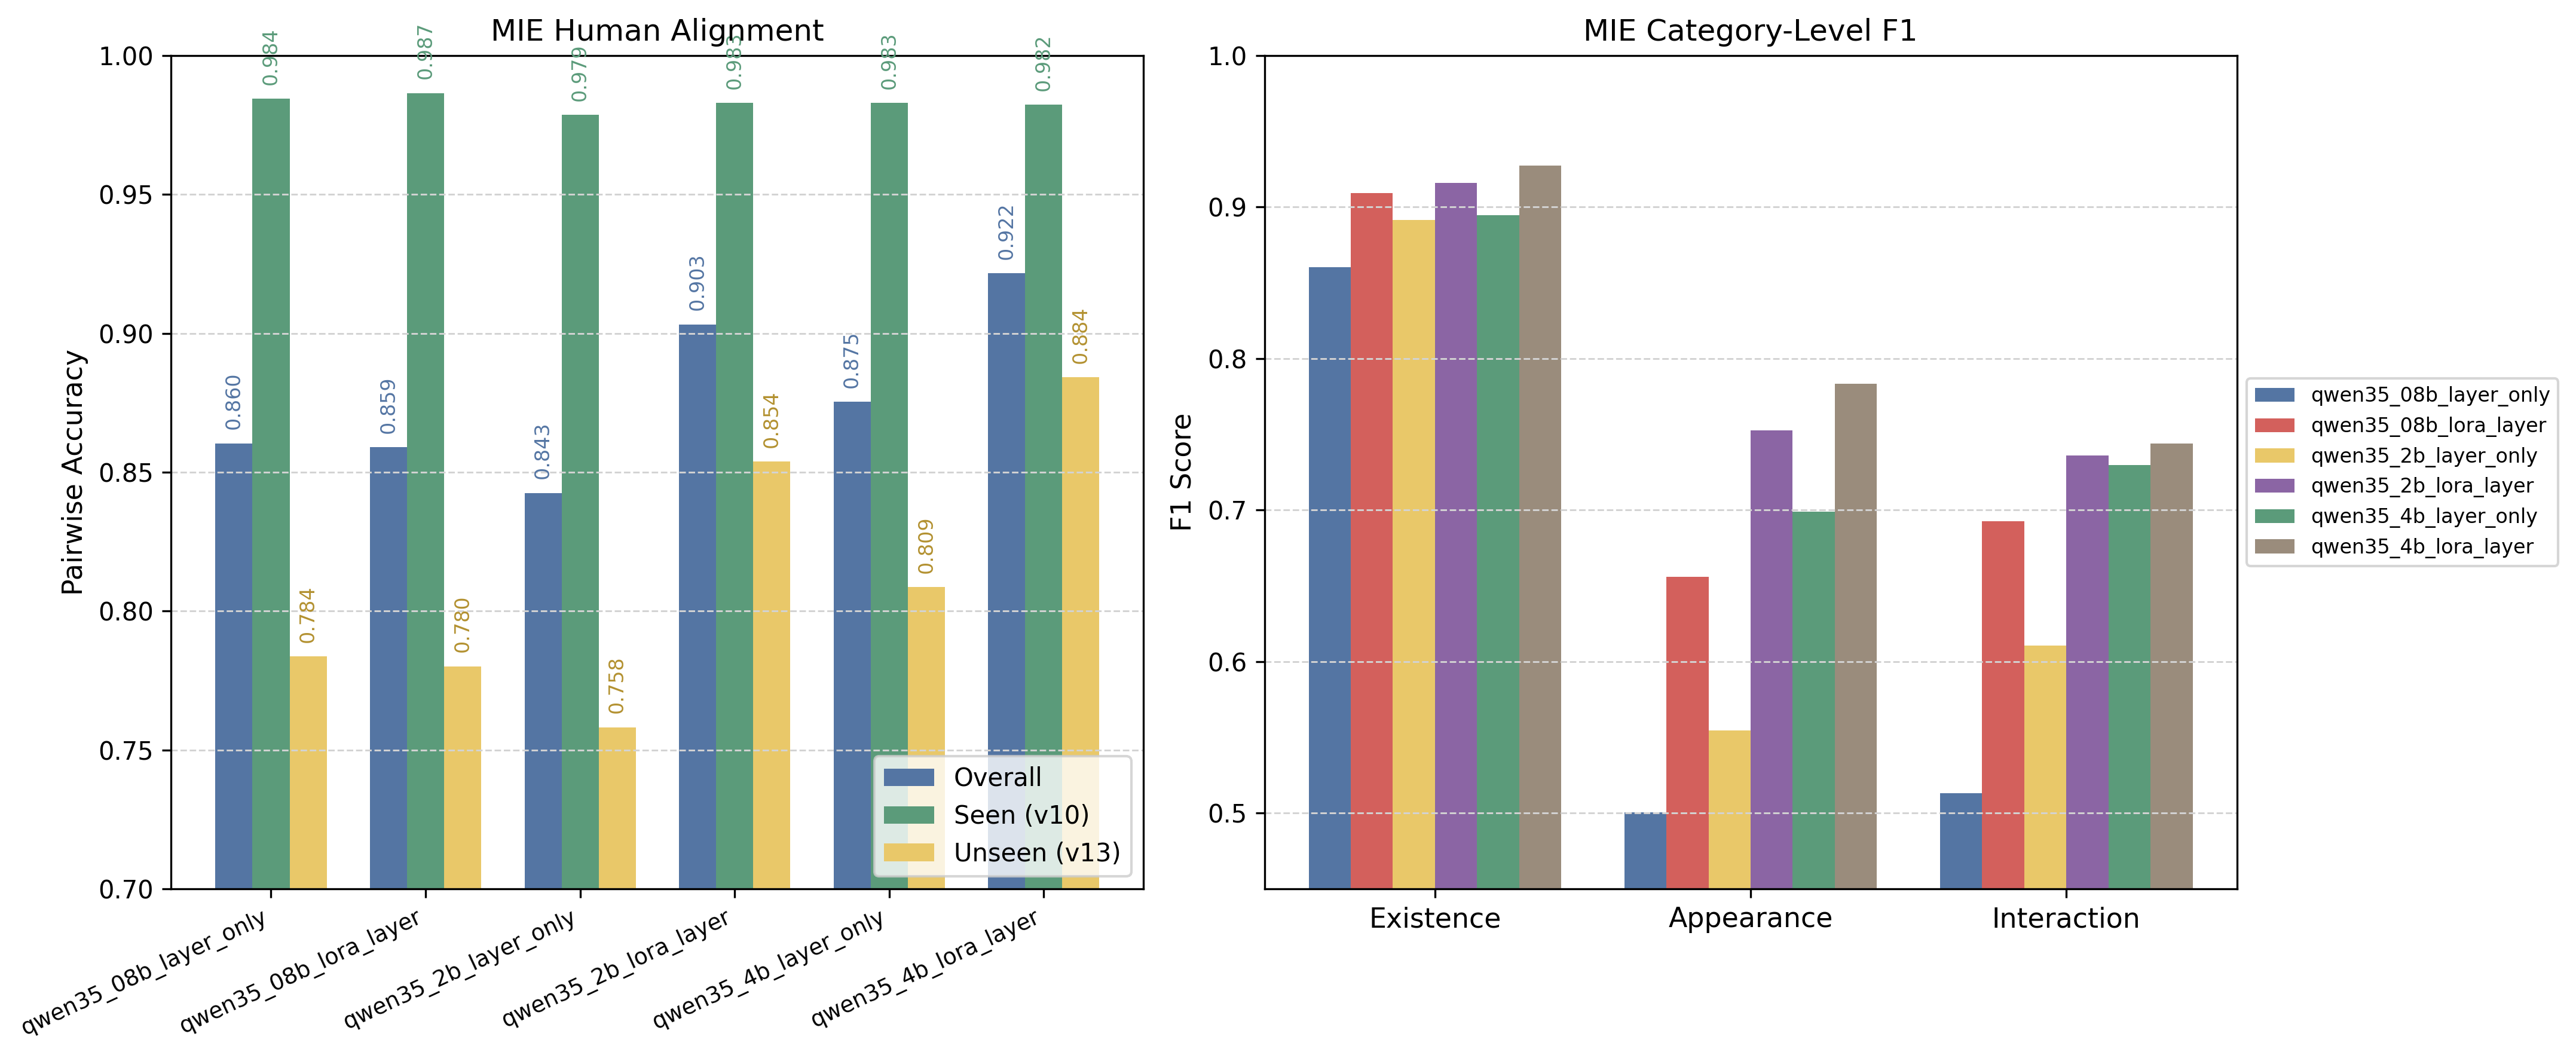
\includegraphics[width=\linewidth]{figures/section_4_2_2_mie_alignment.png}
    \caption{Human alignment of MIE variants on \texttt{MIB-Gold}. Left: overall, seen-generator, and unseen-generator pairwise accuracy. Right: category-level F1 across existence, appearance, and interaction. The 4B LoRA-layer evaluator is the strongest overall model and remains clearly above third-party baselines even on the unseen-generator subset.}
    \label{fig:mie_alignment}
\end{figure}

\paragraph{MIE Breakdown Analysis} We next ask where the gains of the learned evaluator actually come from. A consistent pattern emerges across all six checkpoints: every model performs better on the seen-generator subset than on the unseen-generator subset, confirming that cross-generator generalization remains a non-trivial challenge. However, the size of this gap depends strongly on the tuning regime. The smallest seen-to-unseen drop is achieved by \texttt{qwen35\_4b\_lora\_layer} at $-0.098$, whereas the largest drop appears in \texttt{2b layer\_only} at $-0.221$. This shows that additional model capacity alone is not enough; how that capacity is adapted is equally important.

The LoRA-versus-layer comparison reinforces this conclusion. At 2B, LoRA-layer tuning improves pairwise accuracy by 0.061 and macro-F1 by 0.116 relative to \texttt{2B layer\_only}. At 4B, it still yields gains of 0.046 in pairwise accuracy and 0.044 in macro-F1 over \texttt{4B layer\_only}. Even at 0.8B, where the pairwise gain is nearly neutral, LoRA-layer tuning improves macro-F1 by 0.128. These results suggest that the primary benefit of LoRA-layer tuning is not merely stronger ranking, but consistently sharper diagnostic discrimination.

The category-level breakdown points to the same conclusion. \texttt{Existence} remains the easiest dimension, whereas \texttt{Appearance} and especially \texttt{Interaction} are substantially harder, particularly on the unseen-generator subset. As shown in Figure~\ref{fig:mie_breakdown}, the strongest checkpoint achieves the best balance between overall alignment and fine-grained diagnostic sensitivity under generator shift. Overall, the breakdown analysis clarifies that the best-performing evaluator is not simply the largest model, but the model that combines additional capacity with the right adaptation strategy and preserves diagnostic sensitivity under distribution shift.

\begin{figure}[t]
    \centering
    
\includegraphics[width=\linewidth]{figures/section_4_2_3_mie_breakdown.png}
    \caption{Breakdown analysis of MIE variants. Left: seen-to-unseen generalization gap. Middle: LoRA-layer gains over layer-only tuning at different model scales. Right: category-level F1 for the strongest checkpoint. The results show that LoRA-layer tuning improves diagnostic quality across scales and that interaction remains the hardest binding dimension, especially under generator shift.}
    \label{fig:mie_breakdown}
\end{figure}

\section{Limitations}

\paragraph{Scale and Diversity of the Gold Set} 
While our 4K gold evaluation set was curated under a rigorous double-blind protocol, it inherently captures a finite subspace of the vast combinations of subjects and interactions. 
Specifically, the current benchmark relies on 60 unique reference, which, despite covering major categories, may not fully represent the long-tail distribution of real-world objects and personas. 
Furthermore, the annotator pool may reflect specific aesthetic sensibilities that introduce subtle biases. 
Future iterations will focus on expanding the reference concept library and diversifying the annotator demographics to ensure more robust generalization and equitable evaluation.

\paragraph{Temporal Snapshot of Baseline Generators} 
The MIB gold set reflects the performance of six representative generators at the time of collection. 
Given the rapid velocity of the field, newer architectures may encounter unique failure modes—such as specific multi-modal reasoning bottlenecks—not fully captured by the current distribution. 
To ensure the benchmark’s longevity, we commit to releasing versioned extensions as transformative models emerge, providing a standardized re-annotation protocol to facilitate community-driven growth.

\paragraph{VLM-Induced Noise in the Silver Set} 
The 60K silver set utilizes a VLM-based pipeline for scalable preference pseudo-labeling. Despite its utility, VLM labeling is susceptible to model-specific biases, such as the tendency to conflate surface-level image fidelity with structural binding accuracy. 
Furthermore, these models may underperform on culturally specific concepts underrepresented in their pretraining data. We recommend that practitioners using the silver set for model alignment (e.g., via DPO) treat these labels as high-fidelity but noisy proxies, incorporating human-in-the-loop auditing for safety-critical applications.


\section{Conclusion}
We introduced \textbf{MIBE}, a benchmark-and-metric framework for reference-conditioned multi-subject personalized image generation, centered on the concept of \emph{binding}: the correct assignment of visual identities, appearances, and interactions to their designated subjects.

The primary contribution of this work is \textbf{MIB}, a large-scale, rigorously annotated benchmark constructed via hierarchical prompt design and factorized scene buckets.  
MIB provides (i) a 60K silver training corpus with VLM-derived preference labels and attribute annotations, enabling scalable metric learning and model alignment; and (ii) a 4K gold evaluation set with double-blind human judgments across six state-of-the-art generators, providing a reproducible, human-grounded testbed for future comparisons.  
To our knowledge, MIB is the first dataset specifically designed to isolate and diagnose binding failures at varying subject counts.

Building on MIB, we further propose \textbf{MIE}, a reference-conditioned evaluator that operationalizes binding quality into three interpretable dimensions—Existence, Appearance, and Interaction—alongside a scalar preference signal.  
MIE validates the utility of MIB as a training resource: models trained on the silver set generalize to unseen generators without target-specific fine-tuning, demonstrating that the annotation protocol captures transferable binding signals rather than generator-specific artifacts.

We position MIBE as infrastructure for the multi-subject personalization community.  
The benchmark enables controlled, comparable evaluation across methods; the silver set supports model alignment research; and the diagnostic dimensions provide actionable feedback beyond a single scalar score.  
All data, annotations, and evaluation code will be publicly released under permissive licenses to maximize reproducibility and community uptake.
We hope MIB becomes a standard testbed that accelerates progress on the binding problem and raises the bar for rigorous evaluation in personalized image generation.


\bibliographystyle{plain}  
\bibliography{main.bib}


\newpage
\appendix

\section{Appendix: Human Annotation Observations and Failure Mode Analysis}
\label{sec:appendix_failure_modes}
During the human annotation process for the gold test set, annotators systematically recorded recurring failure patterns across evaluated image pairs. These observations surfaced three consistent and practically significant findings, which we document here to inform future dataset construction and model development efforts.

\paragraph{Failure Rates Increase with Subject Count.}
Annotators consistently found that images depicting a larger number of subjects were significantly harder to evaluate correctly, and that generative models performed more poorly on such cases. The most common failure modes in high-subject-count scenes were subject omission, where one or more individuals were missing from the generated output, and appearance drift, where the physical attributes of individual subjects degraded as the total number of subjects increased. This trend was particularly pronounced for visually similar subjects (e.g., individuals wearing comparable outfits or sharing similar physical features), where models frequently confused or merged identities. Facial attributes and clothing details were identified as the two most error-prone visual channels under these conditions.

% A representative 6-subject, 2-object prompt (ID: 6905) evaluated across four generative models. All models exhibit Existence failures, with subject omission ranging from 1 missing subject (FLUX2, ARK, GPT) to 3 missing subjects (GLM). Appearance drift co-occurs in proportion to the severity of omission, as models compensate for missing identities by blending residual subject features into the remaining figures. This example illustrates a consistent empirical trend: as the number of requested subjects increases, both the frequency and severity of compositional failures escalate across all evaluated models.

\begin{figure}[H]
  \centering
  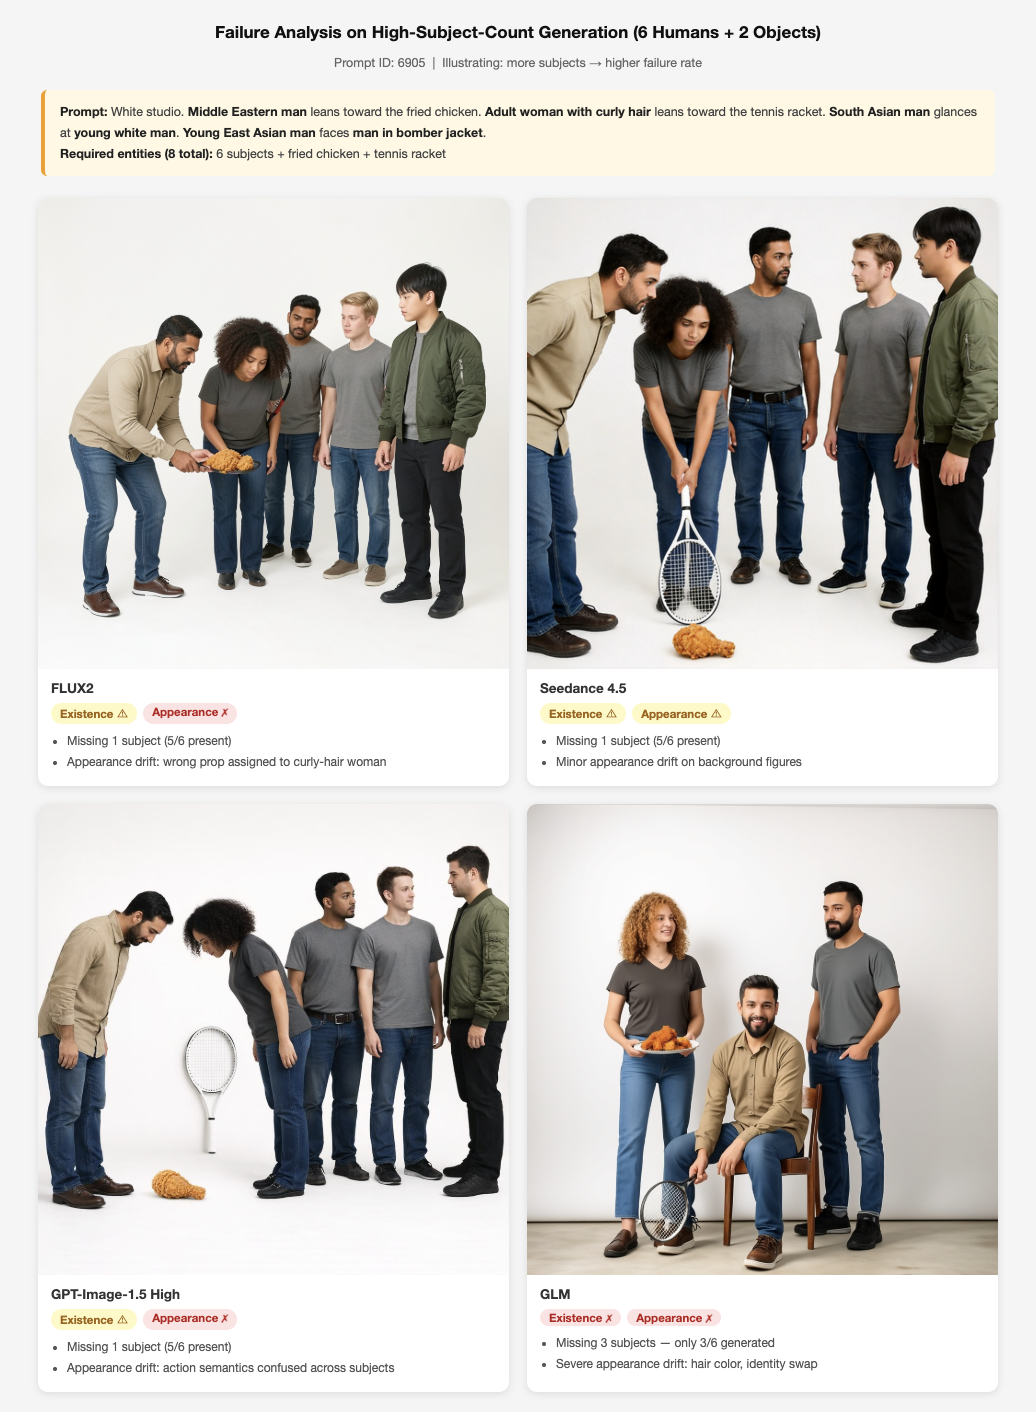
\includegraphics[width=0.75\textwidth]{figures/Appendix-Failure Rates Increase with Subject Count.png}
  \caption{\textbf{Failure Rates Increase with Subject Count} A representative 6-subject, 2-object prompt (ID: 6905) evaluated across four generative models. All models exhibit Existence failures, with subject omission ranging from 1 missing subject (FLUX2, Seedrems-4.5, GPT) to 3 missing subjects (GLM).}
  \label{fig:appendix-failure-rates-subject-count}
\end{figure}

\paragraph{Existence Failures Frequently Co-occur with Appearance Failures.}
A substantial proportion of annotated samples exhibited a systematic co-occurrence between Existence and Appearance failures. When a model fails to render all requested subjects as distinct entities, it often compensates by blending the features of missing subjects into the remaining ones, for instance, combining the facial identity of subject $A$ with the wardrobe of subject $B$ into a single generated figure. This entanglement means that Existence failures are rarely isolated: they tend to cascade into cross-subject feature bleeding, inflating Appearance failure rates in a correlated rather than independent manner. This observation motivates treating the three diagnostic dimensions as structured but not fully orthogonal signals in practice, despite their conceptual independence.

% A representative 4-subject prompt (ID: 32062) generated by Seedream, the best-performing model on this sample. The missing subject (Man in Black Suit) is not simply absent: its visual attributes --- the black tie and formal shirt --- are redistributed onto the surviving Bomber Jacket figure, producing a hybrid identity. This demonstrates that Existence and Appearance failures are structurally coupled: when a subject is omitted, the model tends to absorb its features into remaining figures, making Appearance degradation a systematic downstream consequence of Existence failure rather than an independent error.

\begin{figure}[H]
  \centering
  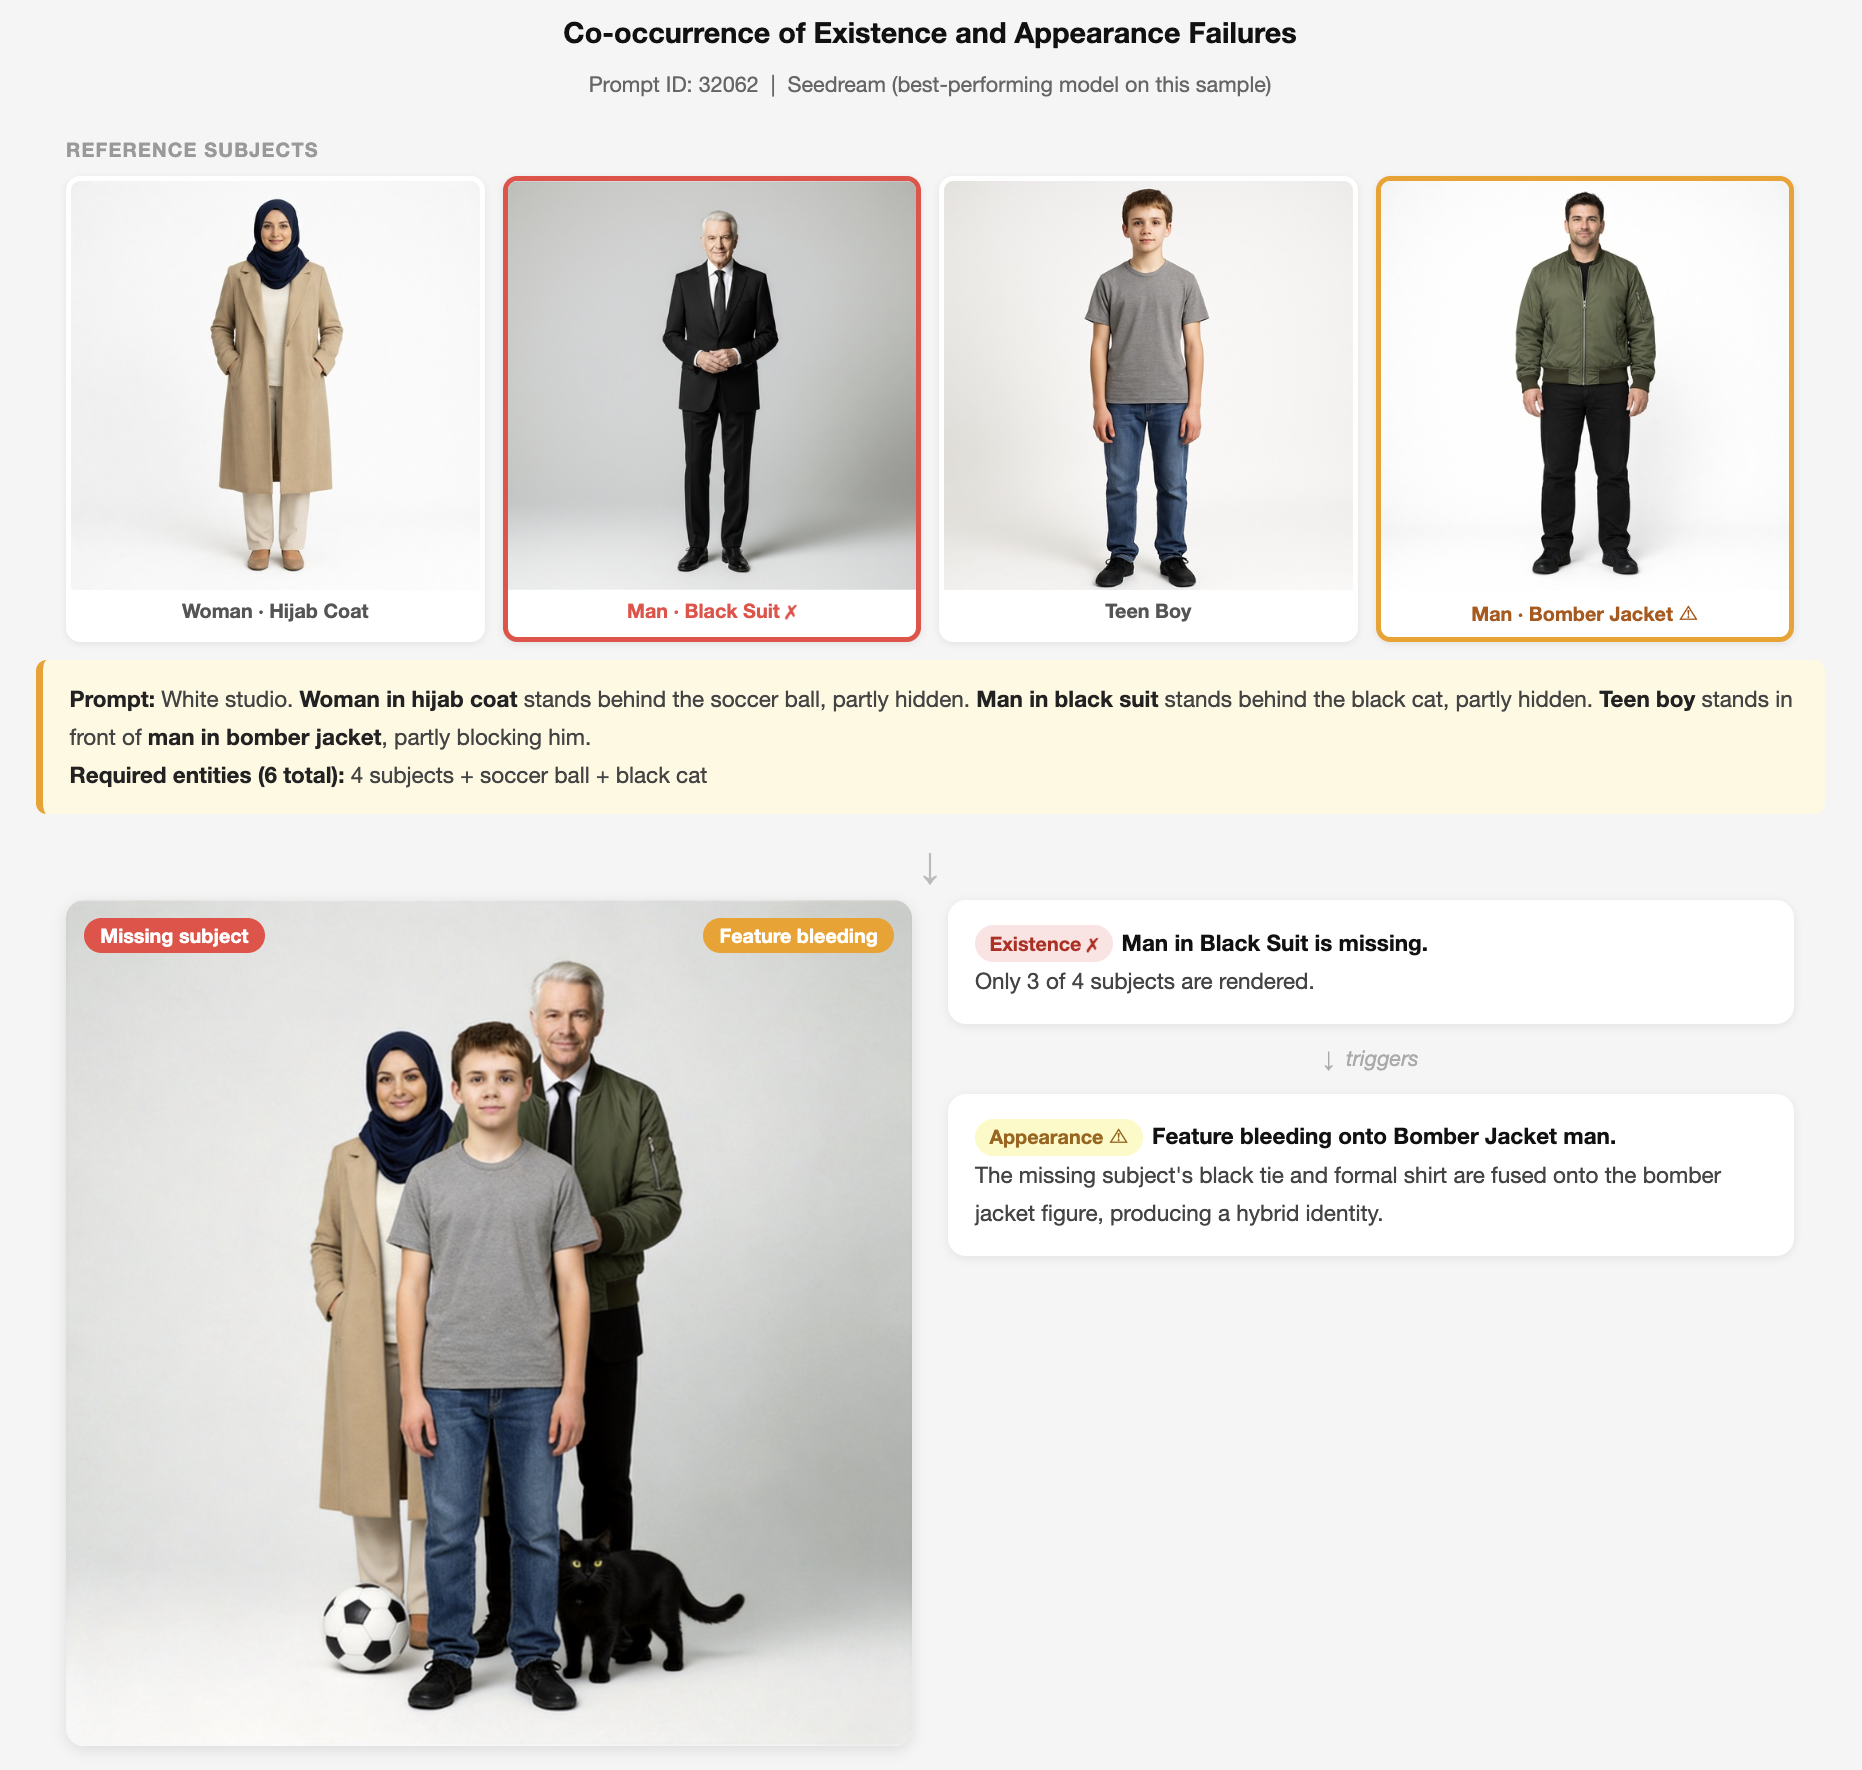
\includegraphics[width=0.8\textwidth]{figures/Appendix-Existence Failures Frequently Co-occur with Appearance Failures.png}
  \caption{\textbf{Existence Failures Frequently Co-occur with Appearance Failures} A representative 4-subject prompt (ID: 32062) generated by Seedream, the best-performing model on this sample. The missing subject (Man in Black Suit) is not simply absent: its visual attributes --- the black tie and formal shirt --- are redistributed onto the surviving Bomber Jacket figure, producing a hybrid identity.}
  \label{fig:appendix-existence-appearance-cooccurrence}
\end{figure}

\paragraph{Multi-Action Overload Leads to Subject Deformation}
Annotators consistently observed that when a single subject is assigned more than one concurrent action or interaction, generative models struggle to faithfully execute all specified behaviors. This overload manifests in two characteristic failure patterns. First, \textit{figure splitting}: the model resolves the conflict by duplicating or fragmenting the subject, distributing distinct actions across two visually similar but non-identical figures — effectively cloning the identity to satisfy each action independently. Second, \textit{action dropout}: the model selectively ignores or partially executes one of the assigned actions, producing a subject that satisfies only a subset of the prompt specification. Both failure modes were reproducible across multiple models and prompt configurations, suggesting that multi-action binding exceeds the compositional capacity of current generative architectures rather than reflecting prompt ambiguity.

\begin{figure}[H]
  \centering
  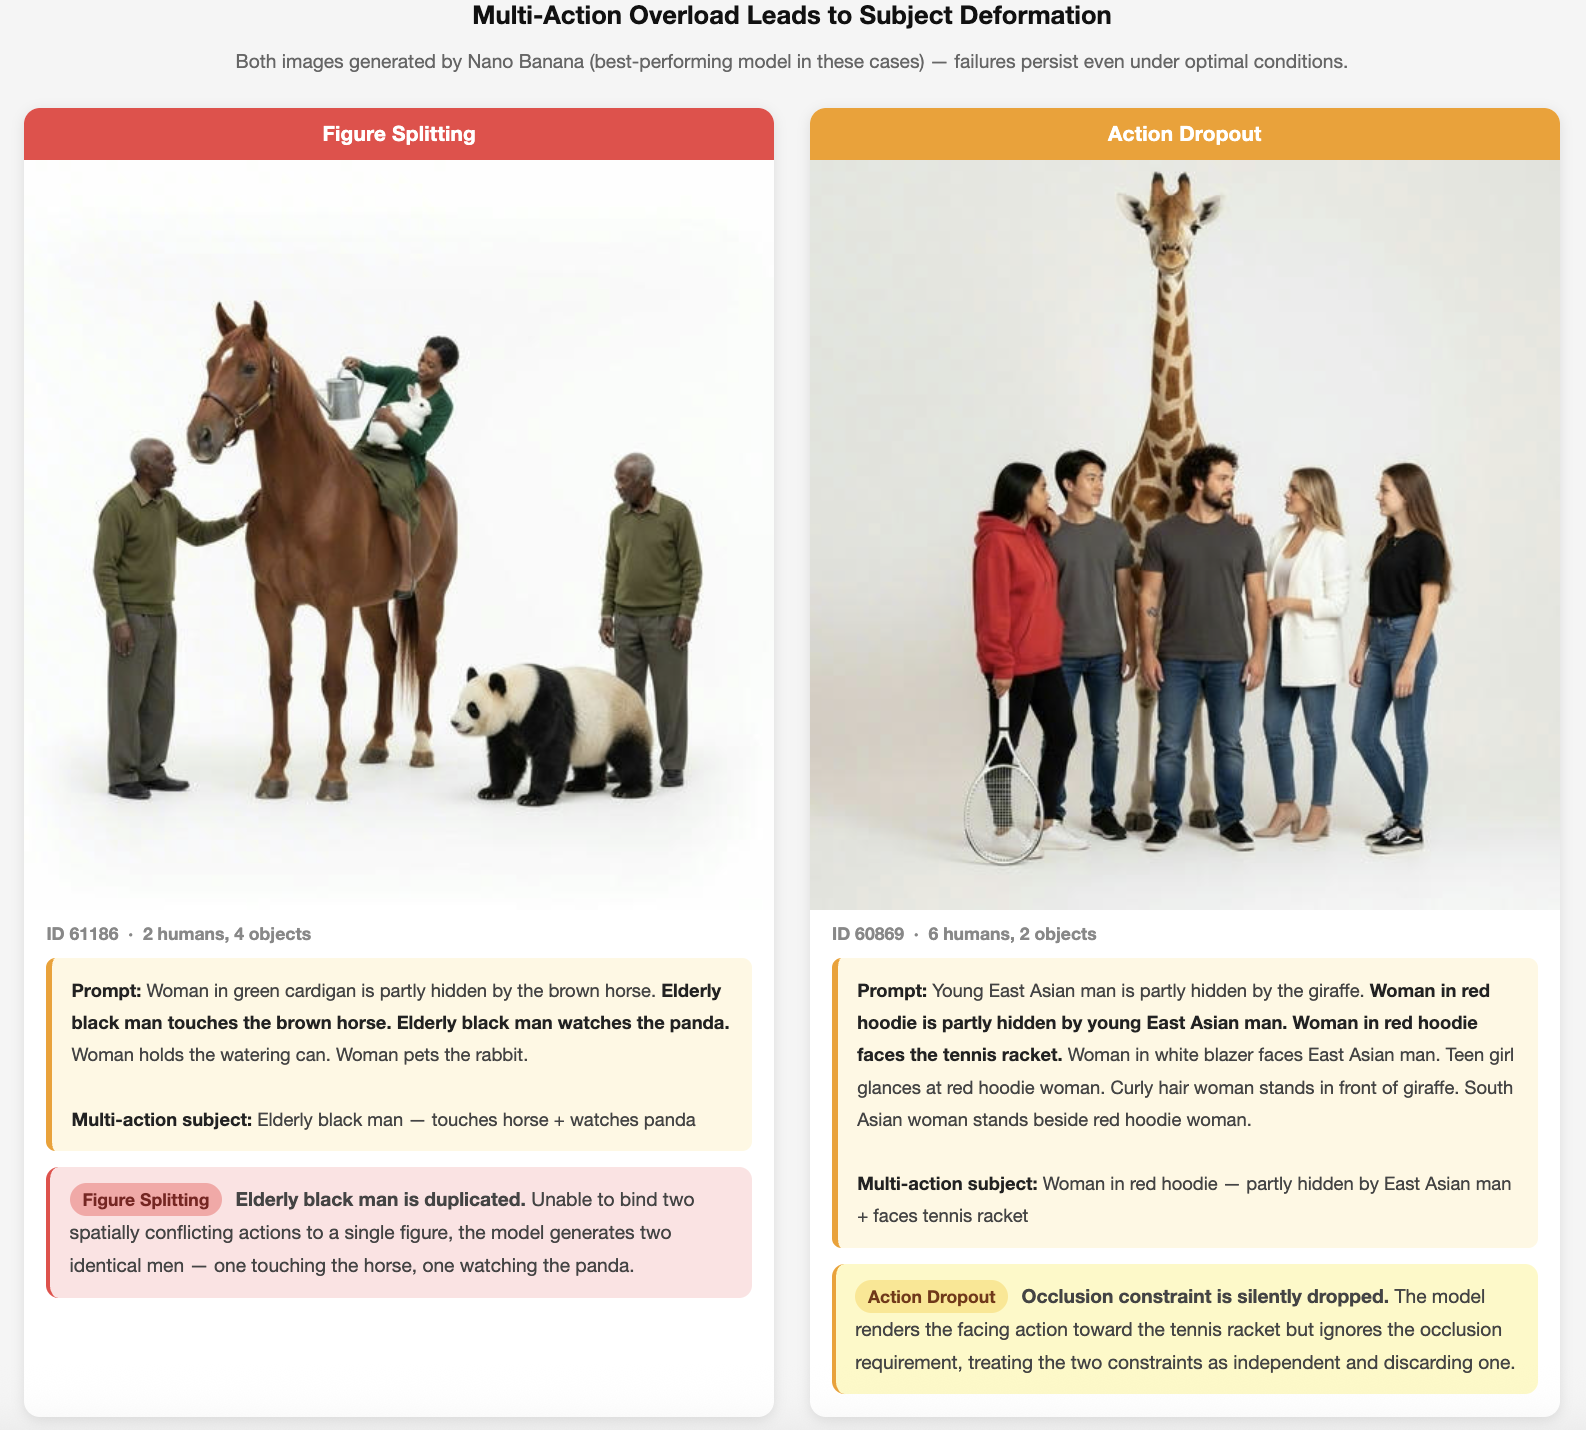
\includegraphics[width=0.7\textwidth]{figures/Appendix-Multi-Action Overload Leads to Subject Deformation.png}
  \caption{\textbf{Multi-Action Overload Leads to Subject Deformation.} When a subject is assigned more than one concurrent action, models either clone the subject to satisfy each action independently (Figure Splitting, ID: 61186) or silently discard one of the assigned actions (Action Dropout, ID: 60869). Both failure modes are observed in Nano Banana, a better performing model in these cases.}
  \label{fig:appendix-multi-action-overload}
\end{figure}

\section{Appendix: SOP Prompt}
\label{sec:app_SOP}
\begin{verbatim}
You are an expert judge for multi-subject personalized image generation.

You will receive:
1. The original generation prompt.
2. Reference images for each subject mentioned in the prompt.
3. Candidate image A.
4. Candidate image B.

Your job consists of two parts:
Part 1: Independent Evaluation
Evaluate candidate A and candidate B independently. For each image, strictly evaluate:
- Existence: Are ALL the required subjects in the references physically present?
  (Generic versions count as 1; completely missing counts as 0).
- Appearance: Are the subjects rendered WITHOUT structural deformations? Do the
  generated subjects strictly match the references across ALL features:
  Face/Skin tone, Hair style, Top clothing, AND Bottoms (pants)?
- Interaction: Does the generated image reflect the described actions, maintain
  correct proportions, and follow realistic spatial/physical laws?

Part 2: Overall Comparison
Compare Candidate A and B and decide the overall winner.

OUTPUT RULES:
- Use ONLY the provided prompt and images.
- All dimensional scores (`*_existence', `*_appearance', `*_interaction') must be
  strictly binary: 1 (fully correct) or 0 (any issue exists).
- `winner' must be either "A" or "B" (Never "Tie").
- Return valid JSON ONLY. Absolutely NO markdown formatting.
- CRITICAL: To focus on errors, the JSON MUST begin with `a_flaw_log` and
  `b_flaw_log`. DO NOT list perfect subjects. ONLY list subjects with errors and
  explicitly state what is wrong (Missing, Wrong Face/Hair/Skin, Wrong Top,
  Wrong Pants, Action/Spatial/Physics Error). If an image is 100% perfect,
  write "None".

SCORING NOTES & SPECIFIC EDGE CASES:
- Appearance (Strict Identity & Wardrobe): You MUST check the whole person. If a
  subject has the correct top but wrong pants, wrong hair, or mismatched skin
  tone/face compared to the reference, score Appearance as 0 and log the
  specific flaw (e.g., "Woman red hoodie: Wrong face/skin color",
  "Man flannel shirt: Wrong pants color").
- Appearance (Mangled/Melted): Any structural artifacts (extra limbs, mangled
  faces) = Appearance 0.
- Existence vs Appearance: If requested "man denim jacket" is drawn as a generic
  man in a grey sweater, Existence is 1, Appearance is 0.
- Interaction (Partial): Evaluate interactions based ONLY on rendered subjects.
  If an interaction requires a missing subject, Interaction is 0.
- Interaction (Physics, Environment & Scale): Obvious physical violations
  (e.g., objects floating in mid-air without support) OR severe scale distortions
  between objects (e.g., abnormally giant bread, miniature people) = Interaction 0.
  HOWEVER, the presence of unprompted but logical supporting structures
  (e.g., tables, pedestals) used to hold objects is PERMITTED and should NOT be
  penalized.

EXPECTED JSON SCHEMA:
{
  "a_flaw_log": "Middle eastern man: Appearance (wears green sweater instead of
  beige shirt). Man flannel shirt: Appearance (wrong pants color). Woman red
  hoodie: Appearance (mismatched face/skin/hair). Interaction: Man is not
  occluded by the woman; The burger is floating in mid-air.",
  "b_flaw_log": "Middle eastern man: Missing. Man bomber jacket: Missing. DSLR
  camera: Missing. Interaction: Man is not walking towards/staring at the woman;
  Fails due to missing interaction targets.",
  "a_existence": 1,
  "a_appearance": 0,
  "a_interaction": 0,
  "b_existence": 0,
  "b_appearance": 0,
  "b_interaction": 0,
  "winner": "A"
}
\end{verbatim}

\newpage
\section{Appendix: Demos of Generated Training Labels}
\label{sec:app_SOP_demo}

\begin{figure}[H]
    \centering
    \begin{subfigure}[b]{0.46\textwidth}
        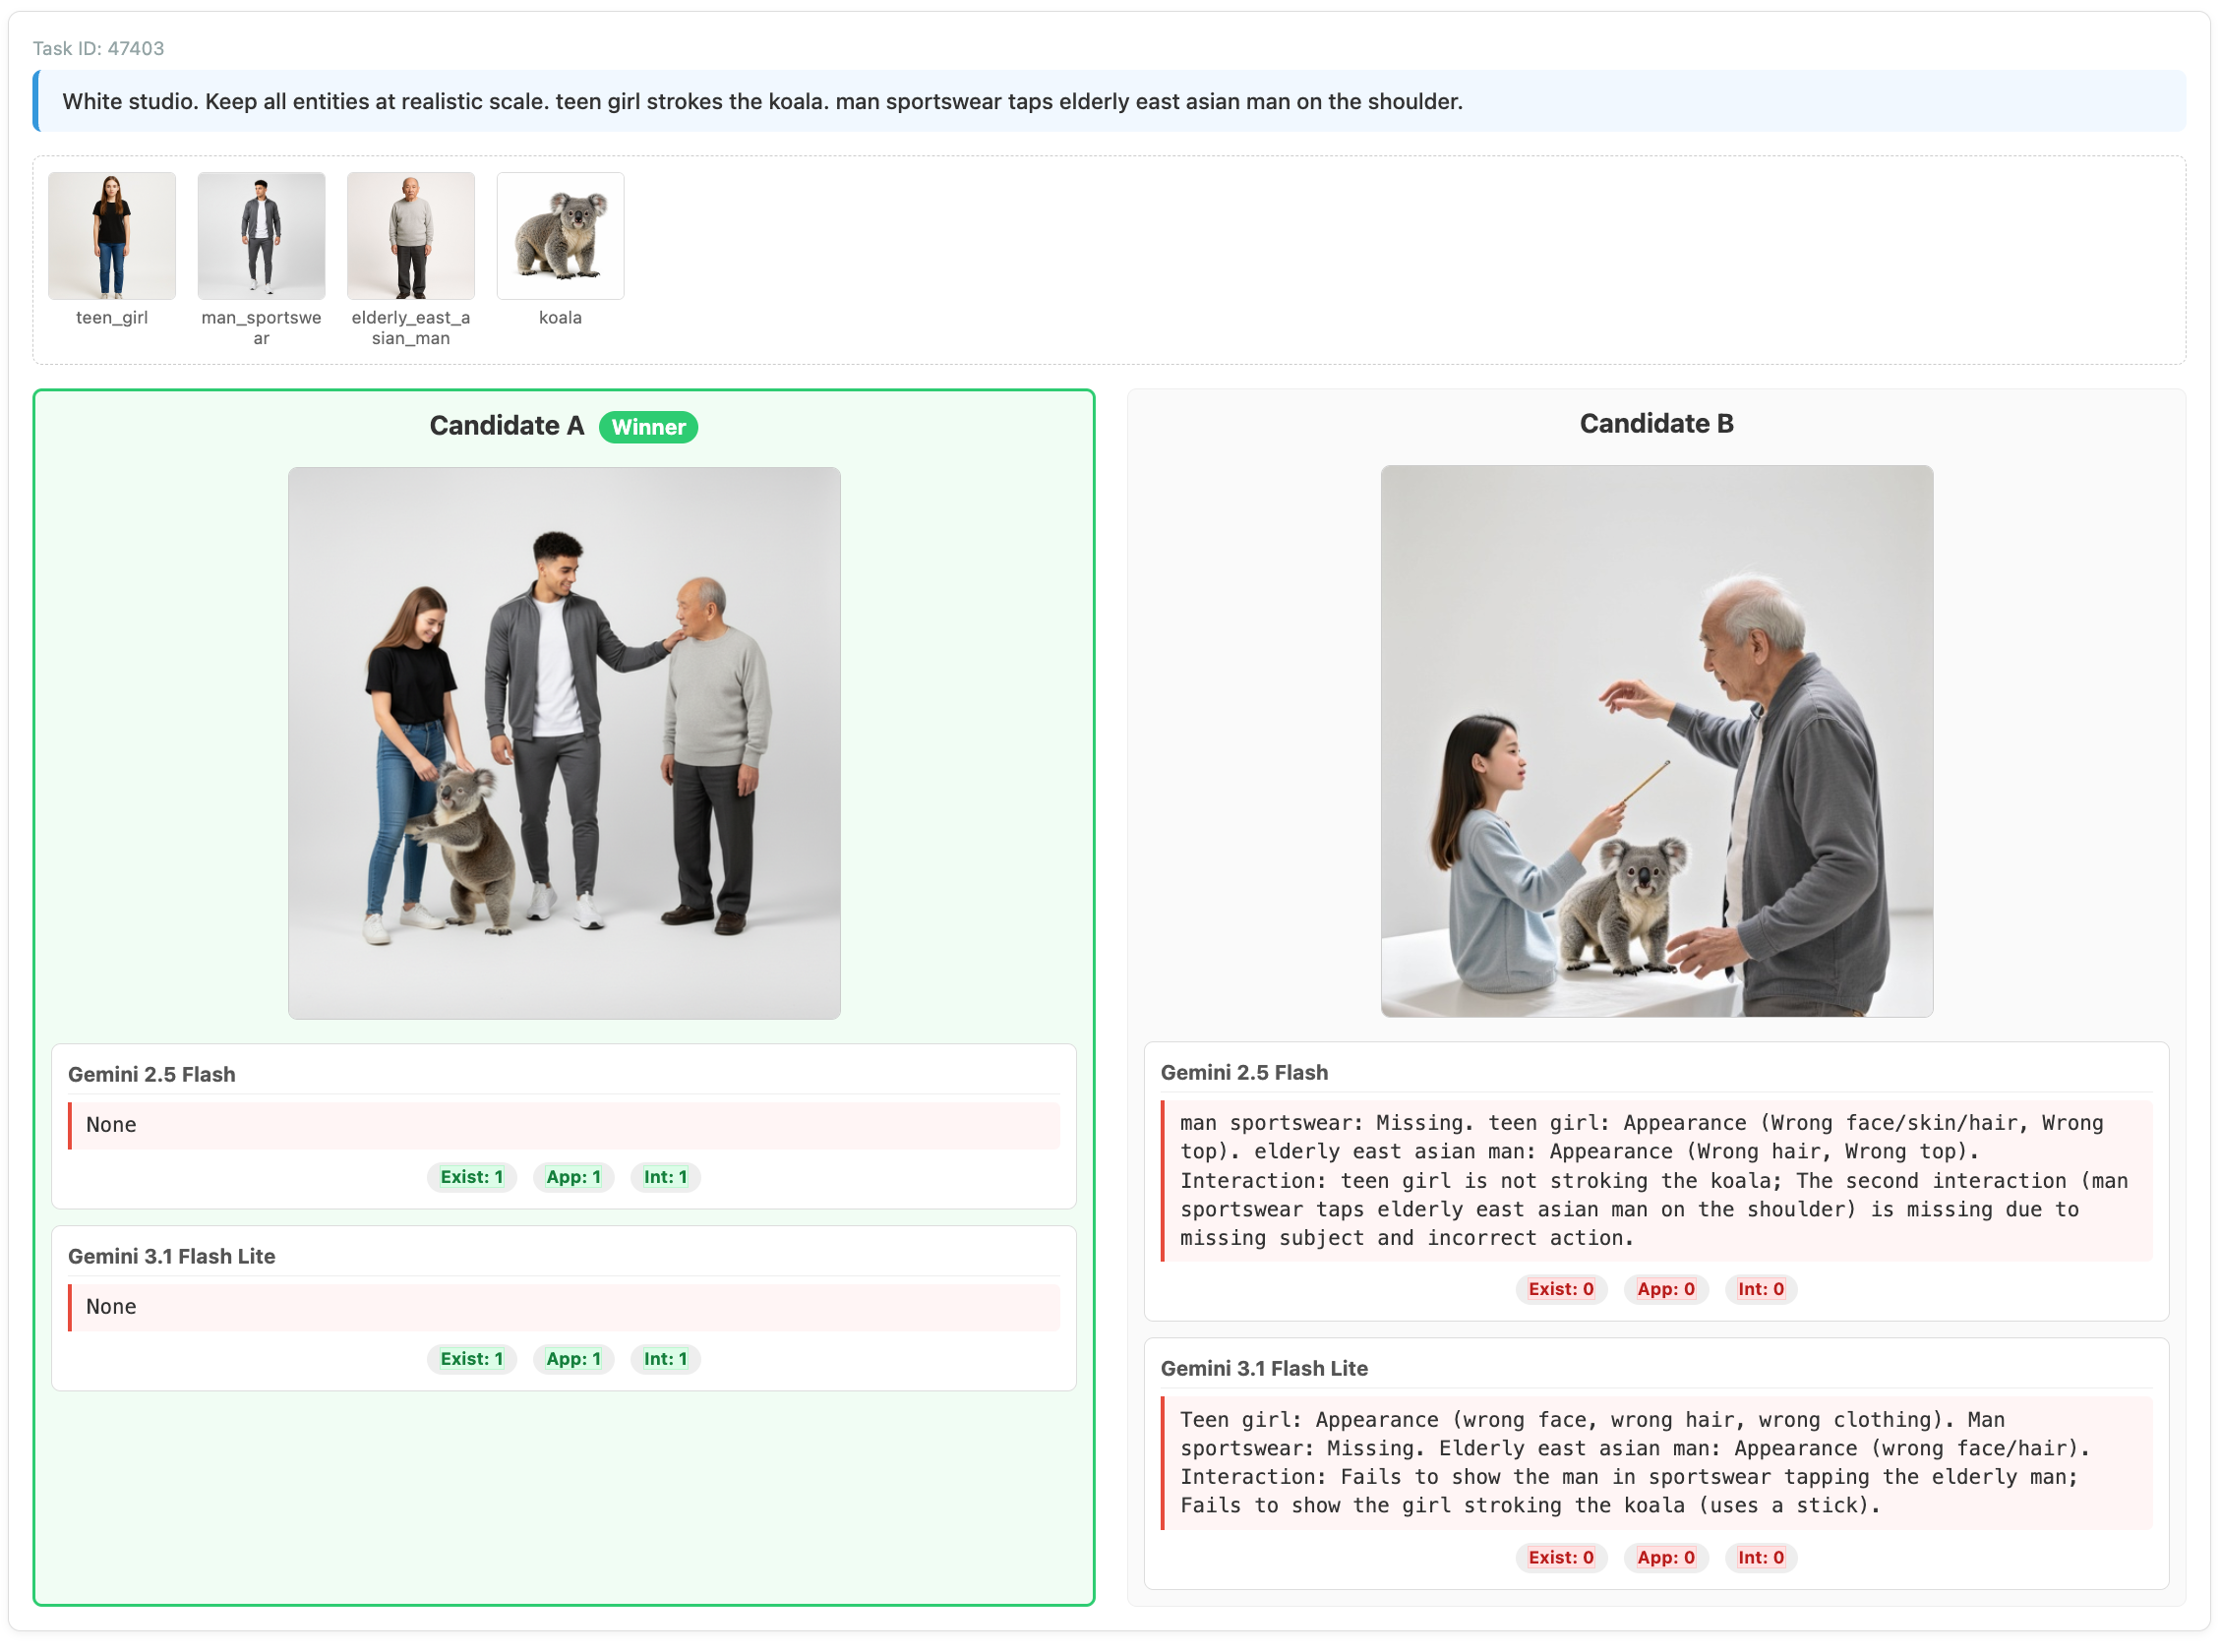
\includegraphics[width=\textwidth]{figures/SOP_demo_1.png}
        \caption{Action and Target Errors}
    \end{subfigure}
    \hfill
    \begin{subfigure}[b]{0.46\textwidth}
        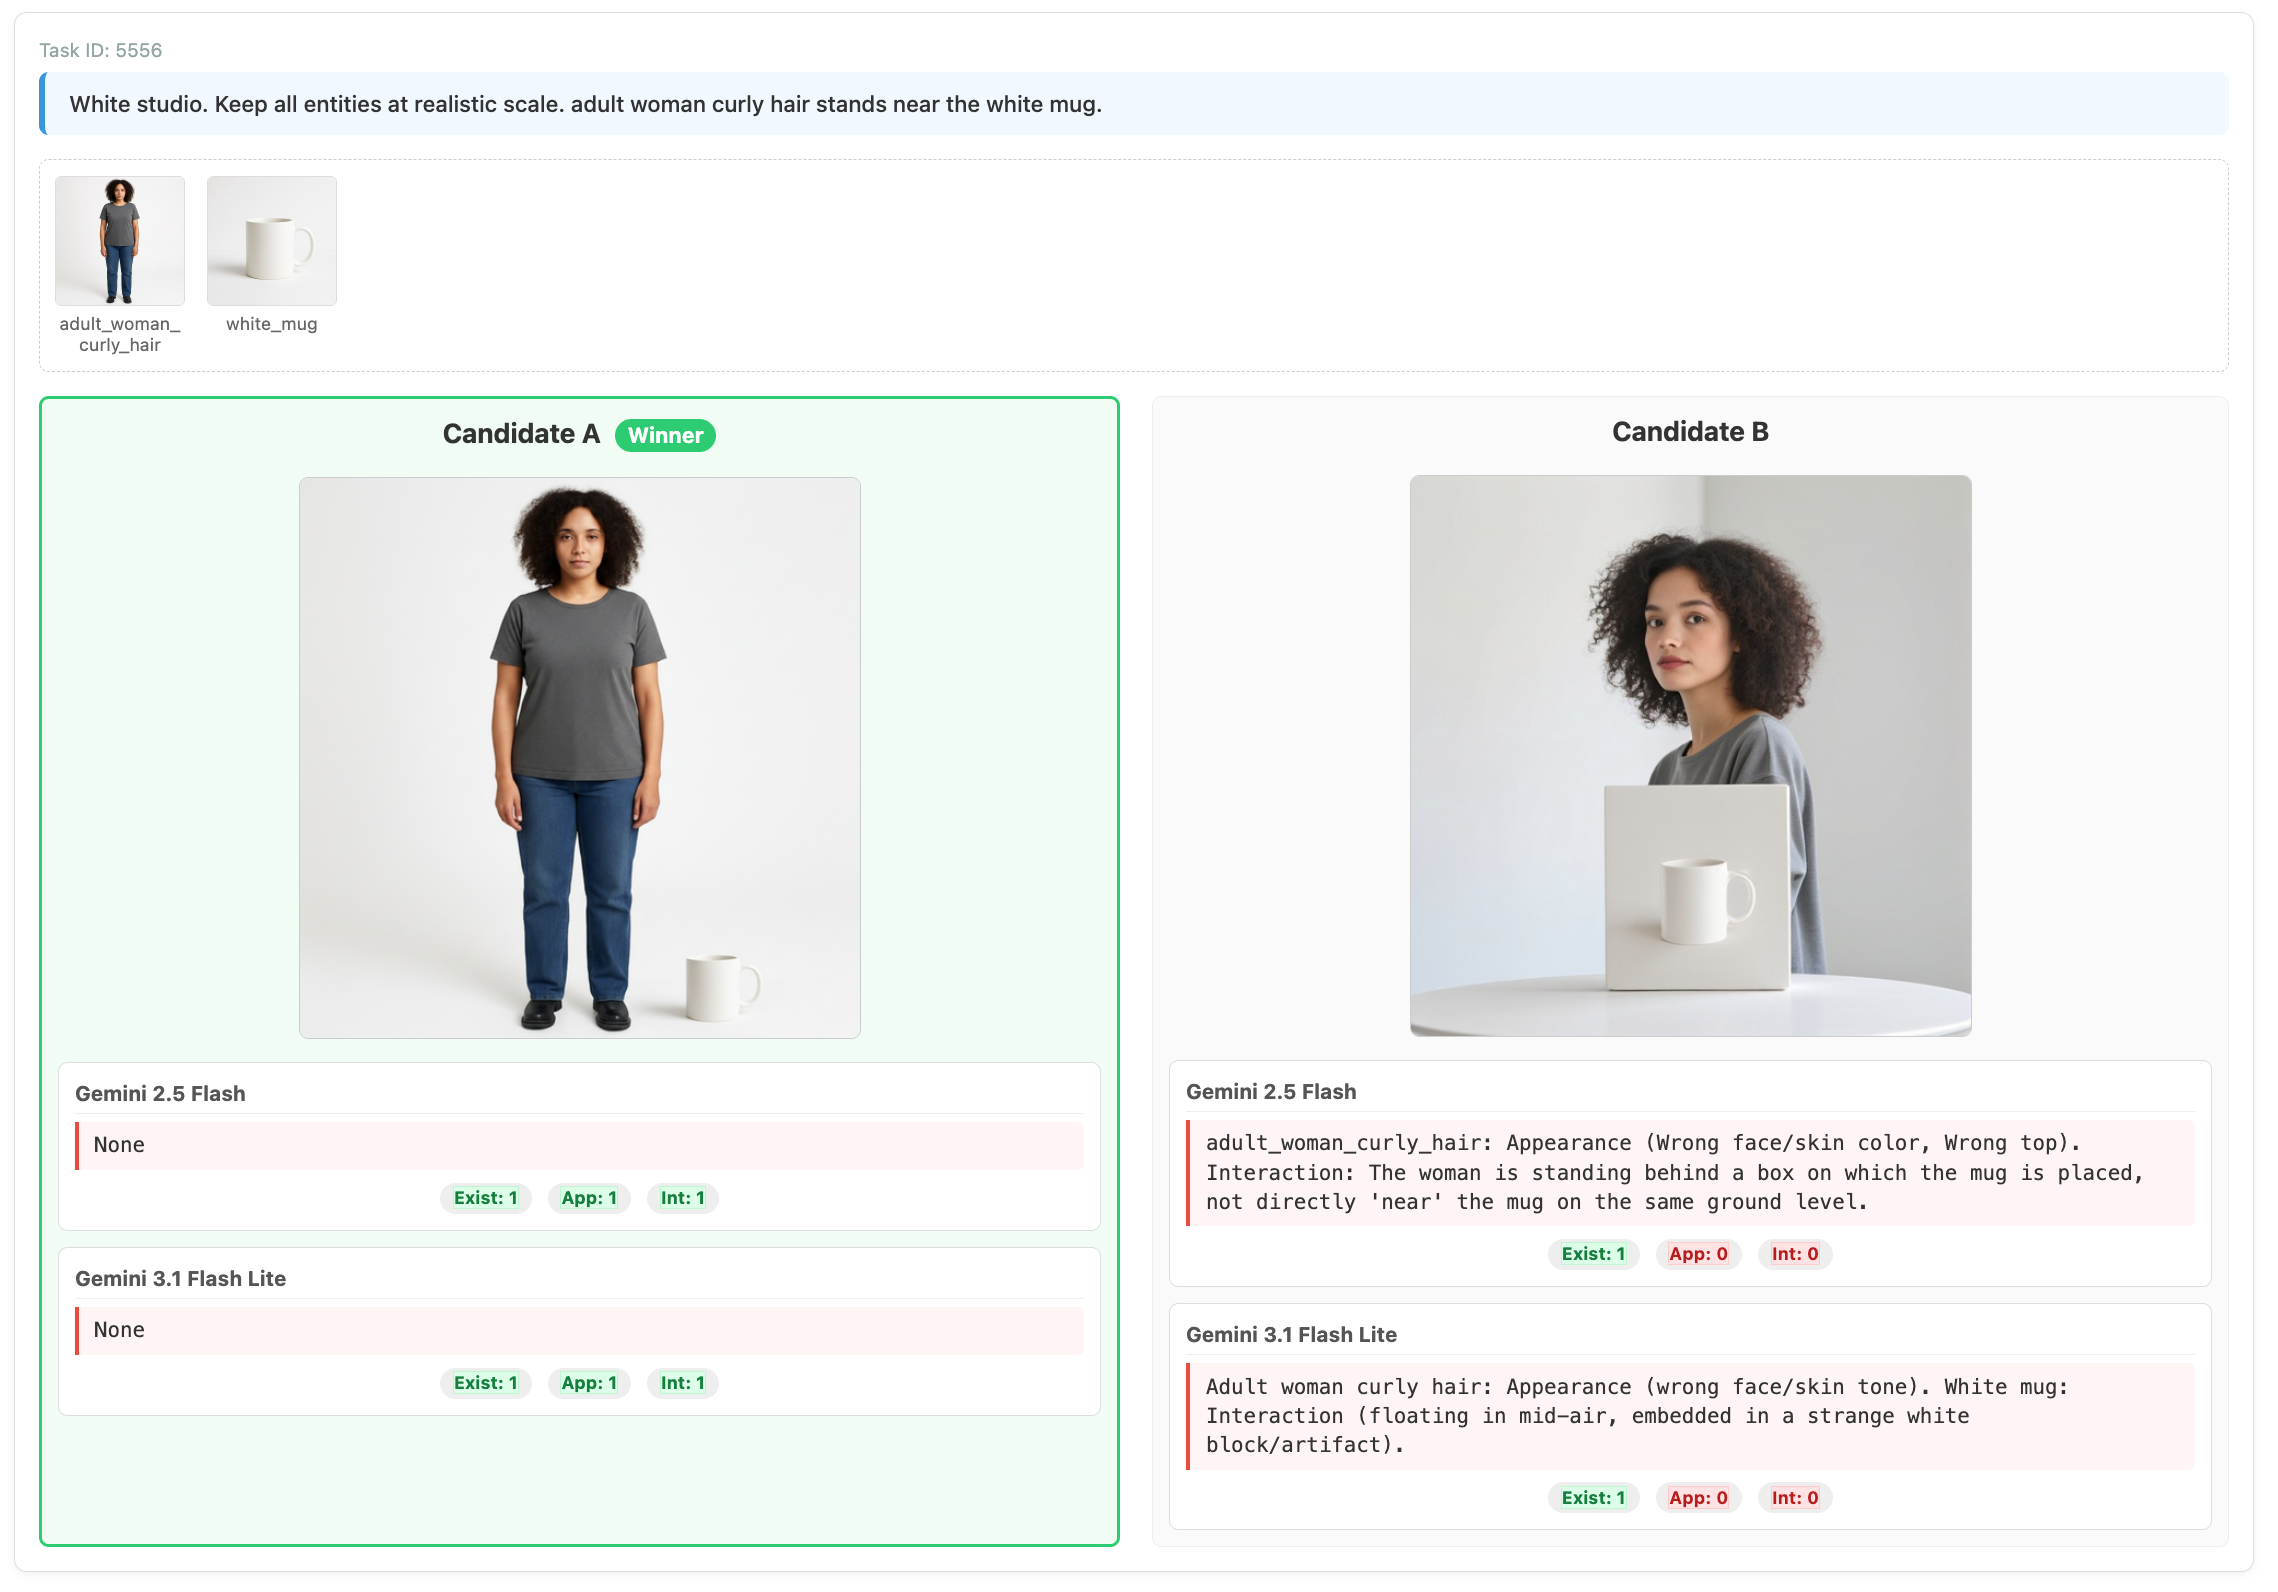
\includegraphics[width=\textwidth]{figures/SOP_demo_2.png}
        \caption{Physics and Spatial Violations}
    \end{subfigure}
    \vspace{1em}
    \begin{subfigure}[b]{0.46\textwidth}
        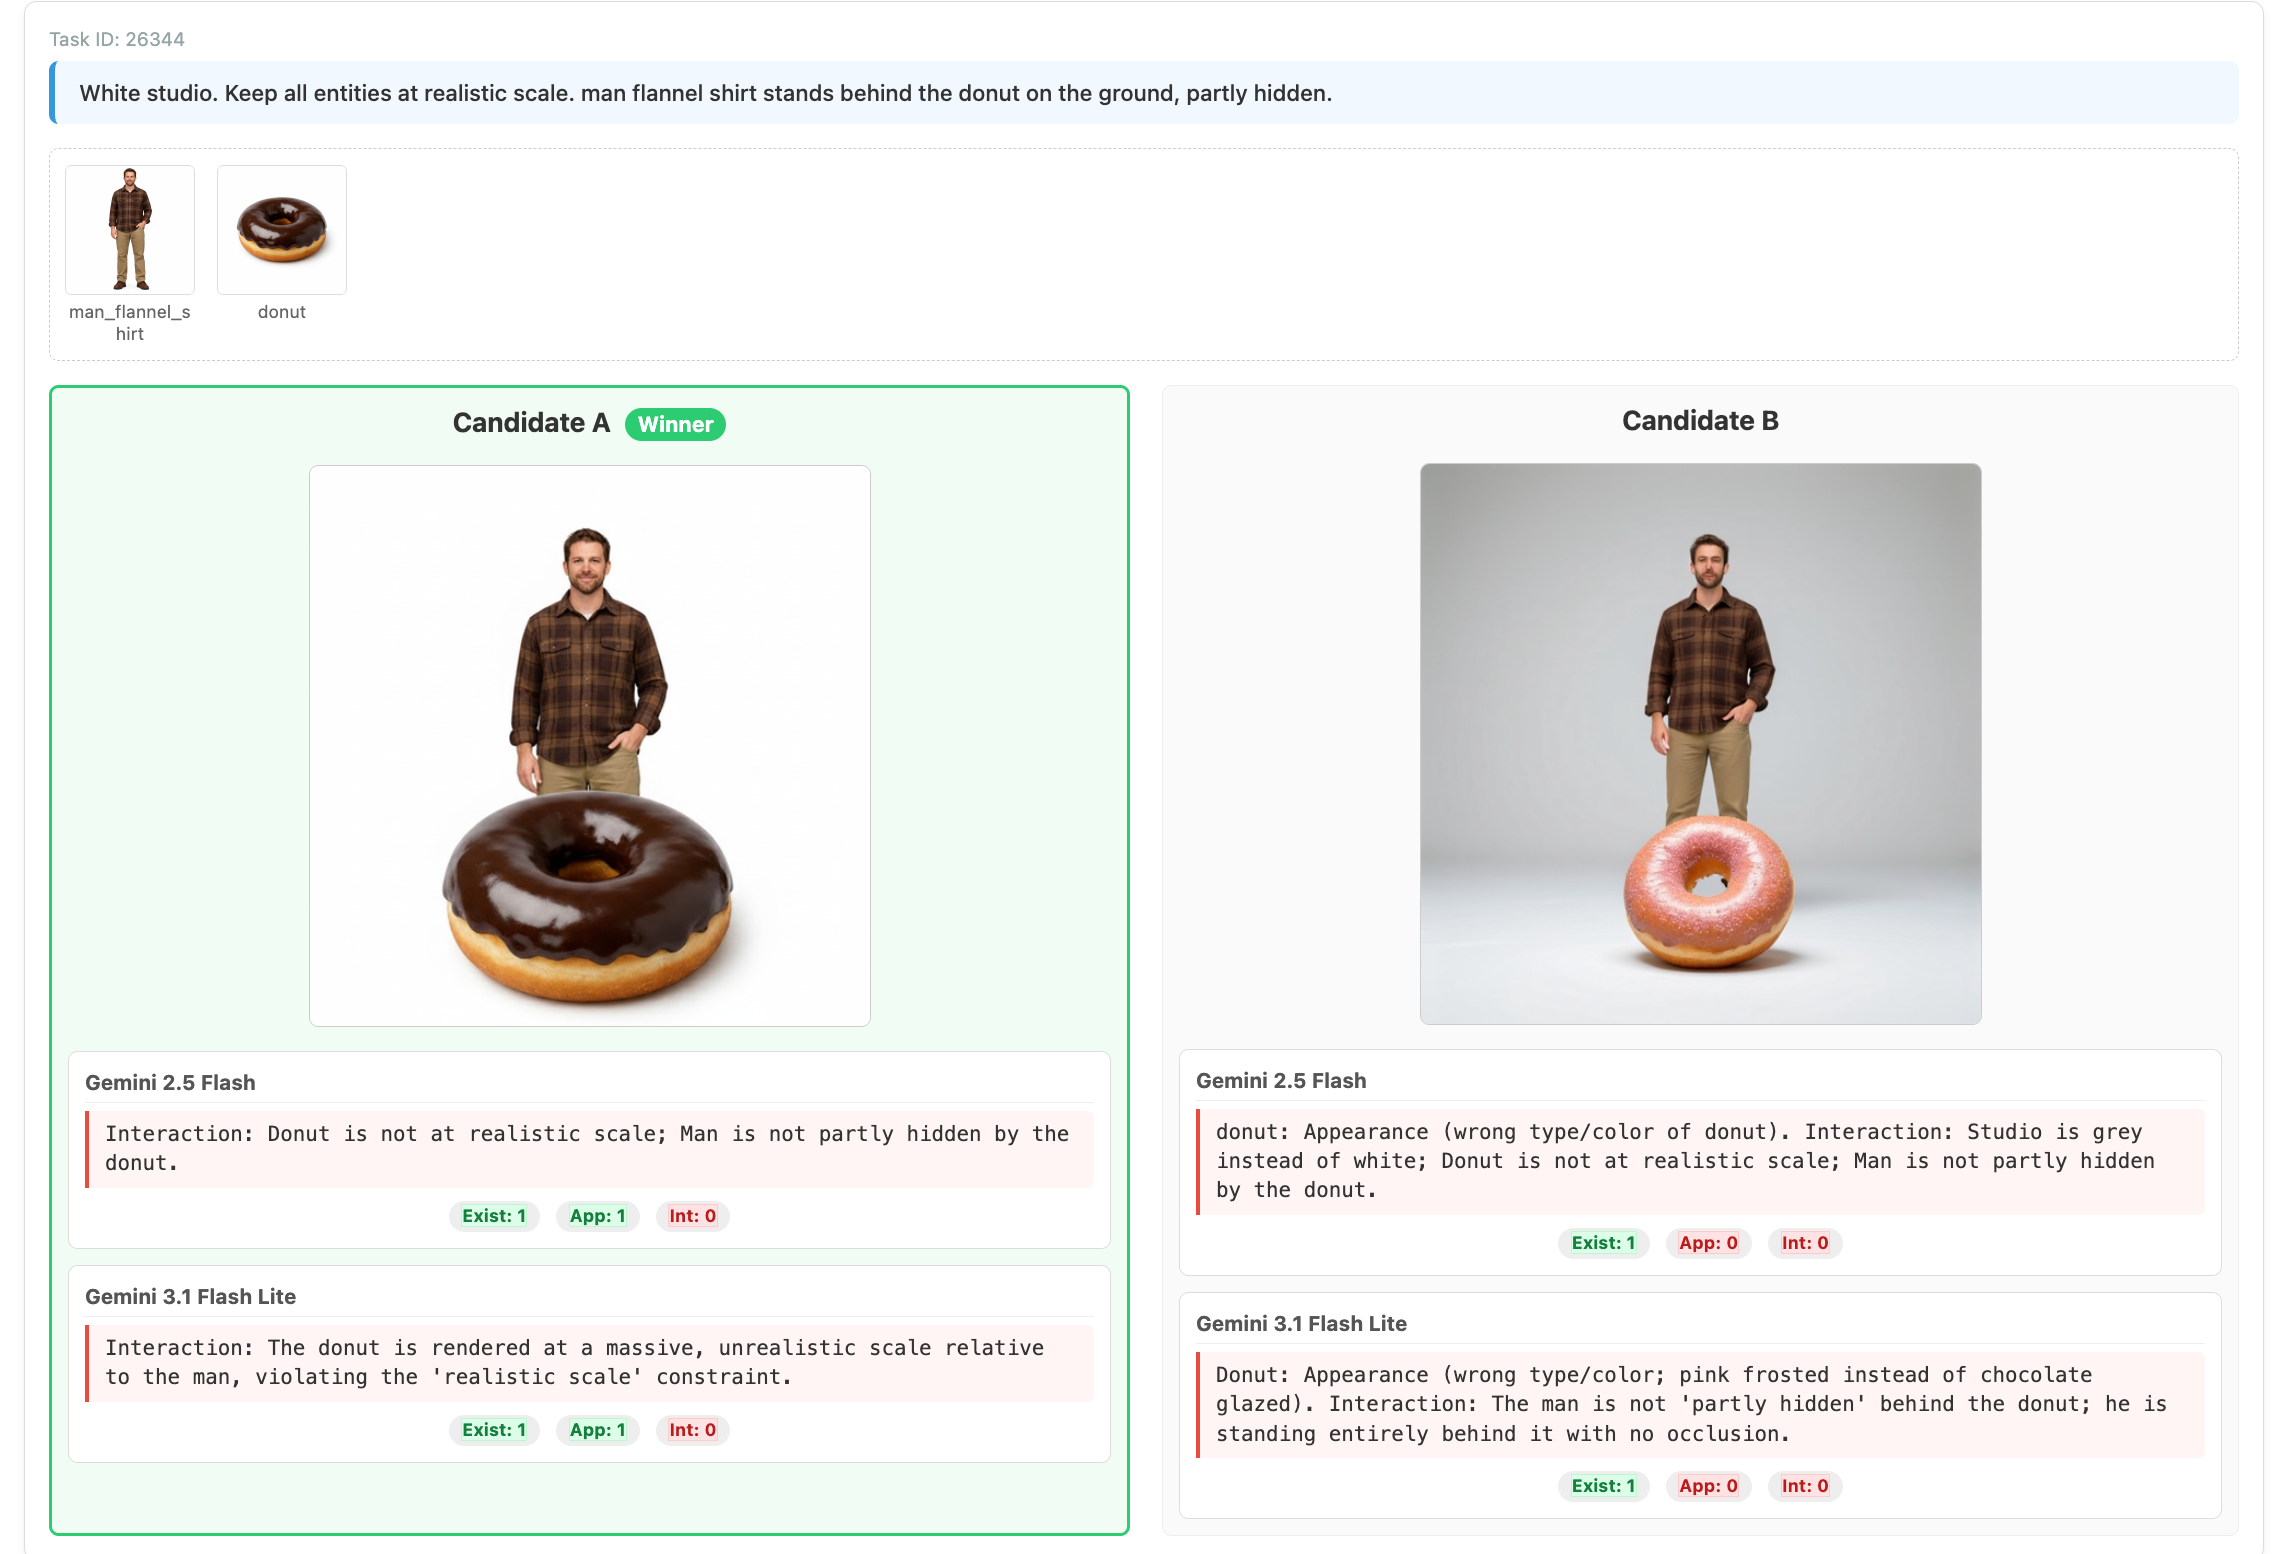
\includegraphics[width=\textwidth]{figures/SOP_demo_3.png}
        \caption{Appearance and Occlusion Errors}
    \end{subfigure}
    \hfill
    \begin{subfigure}[b]{0.46\textwidth}
        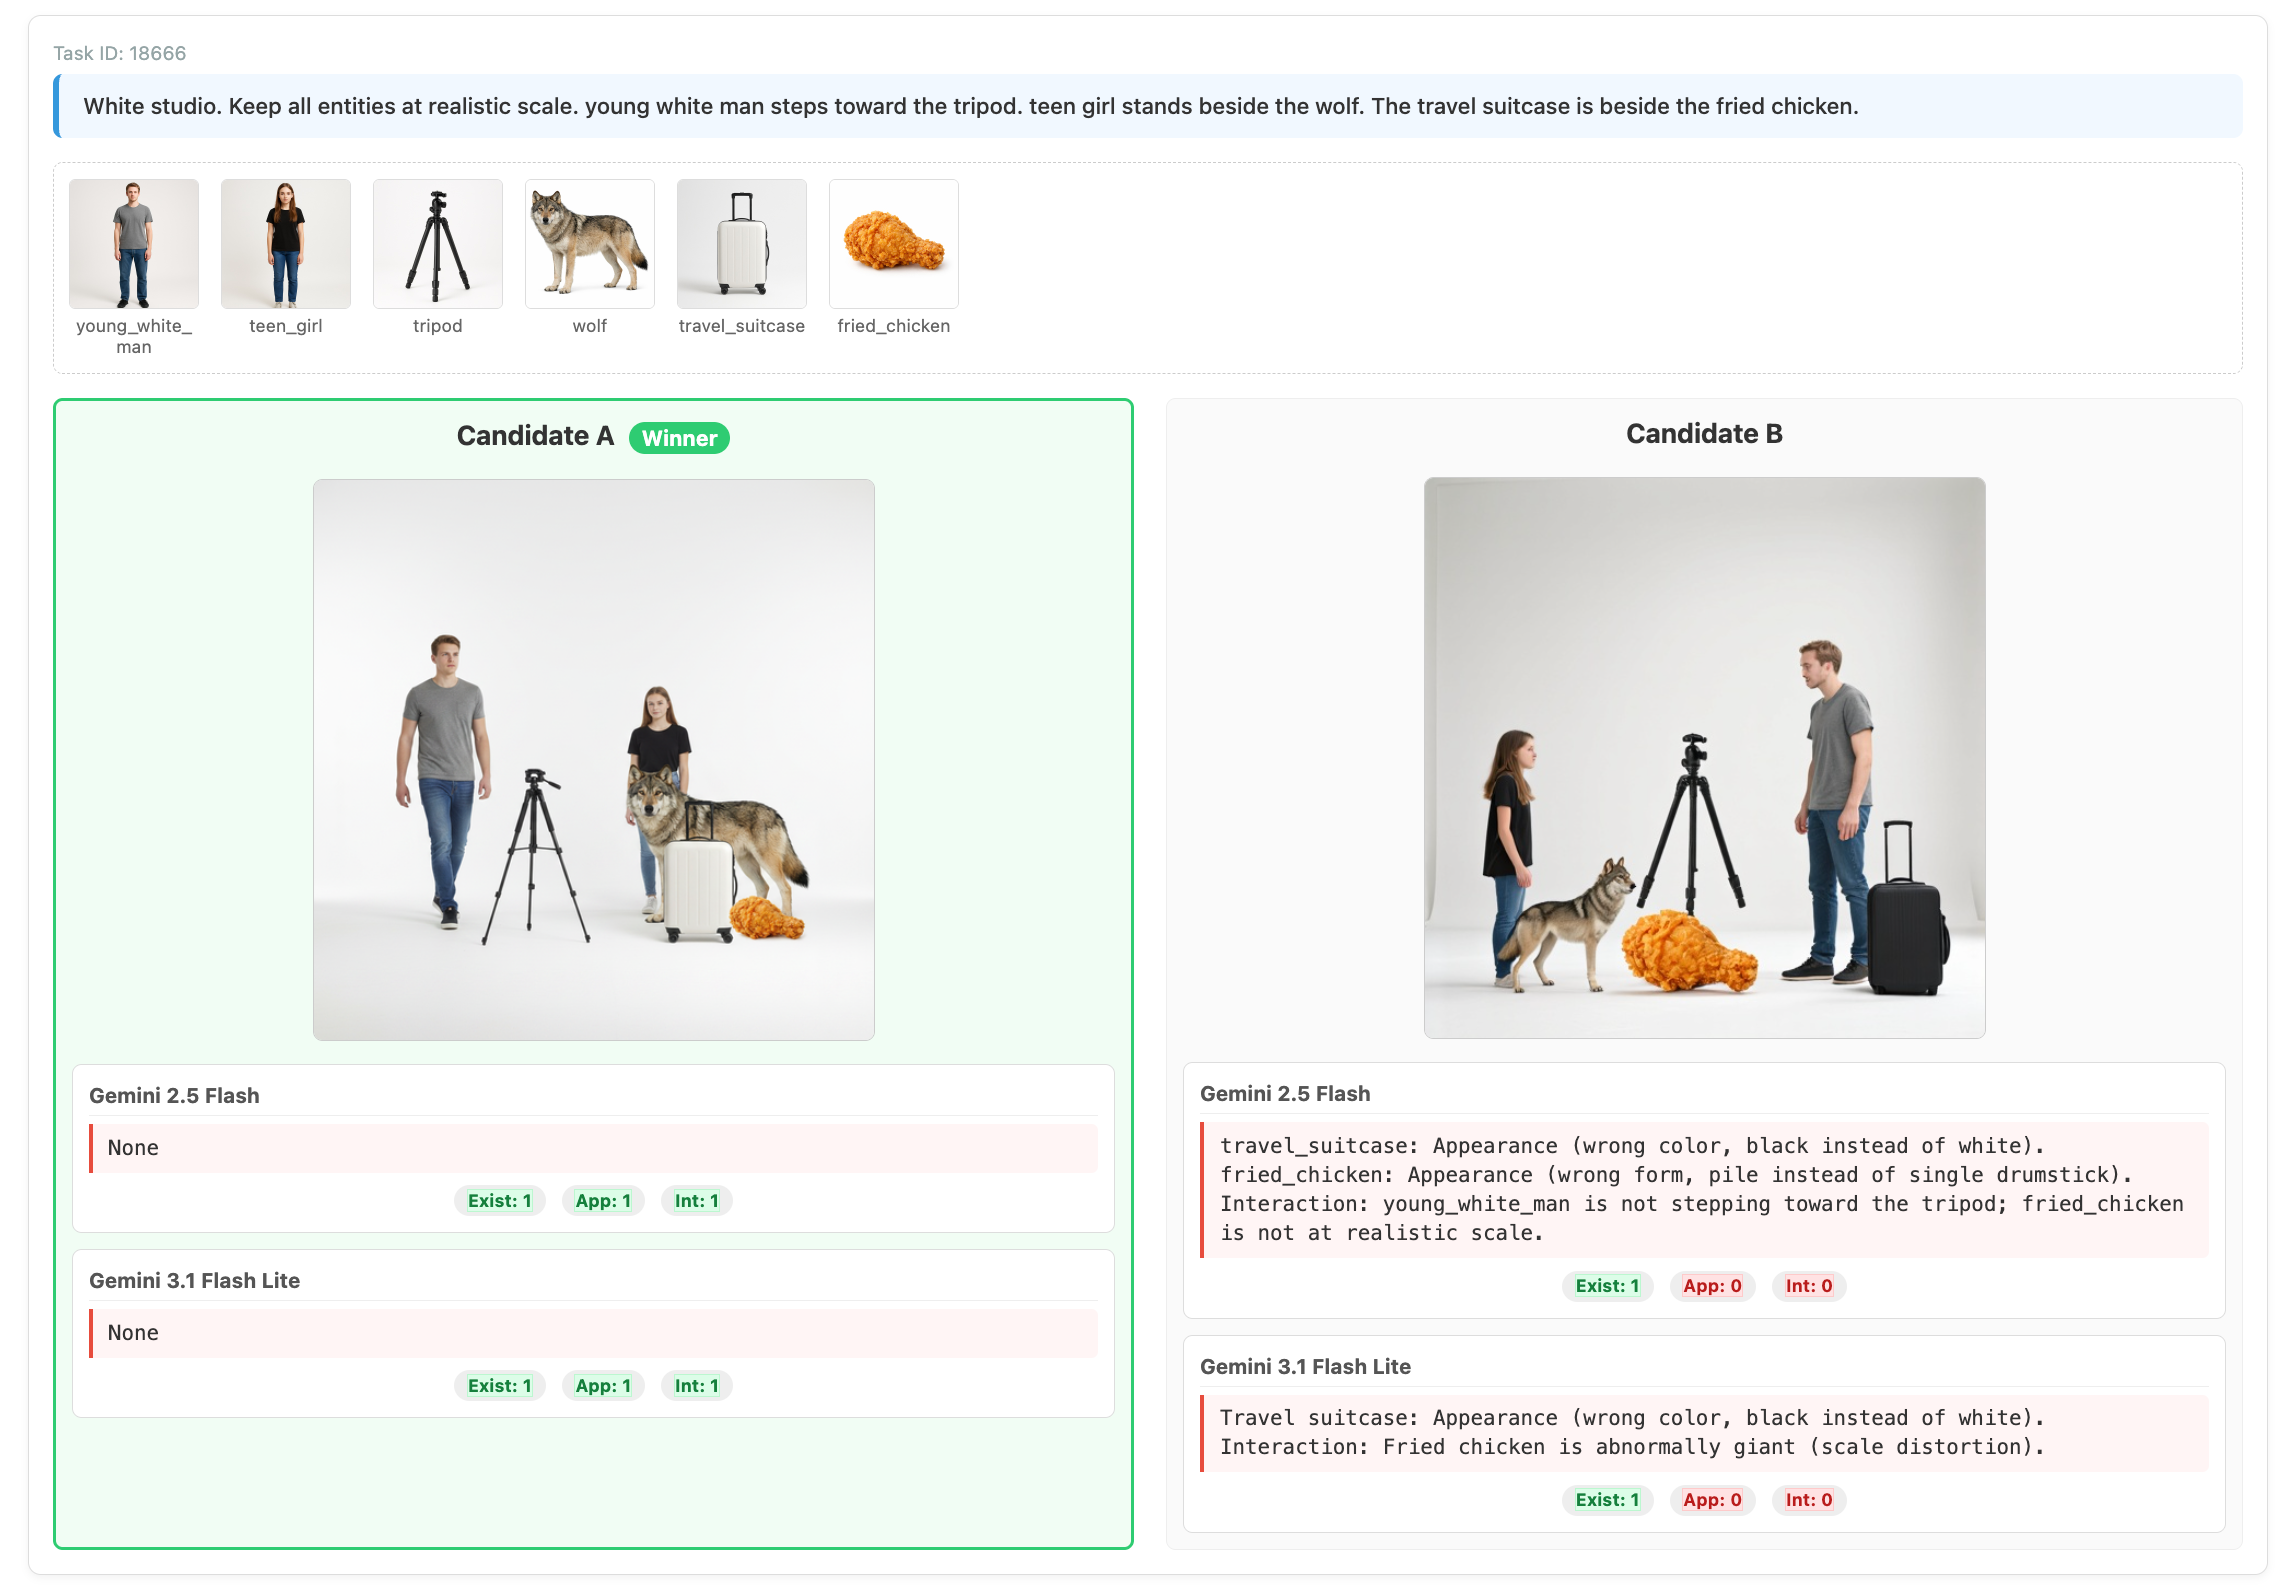
\includegraphics[width=\textwidth]{figures/SOP_demo_4.png}
        \caption{Scale Distortion and Color Mismatch}
    \end{subfigure}
    \vspace{1em}
    \begin{subfigure}[b]{0.8\textwidth}
        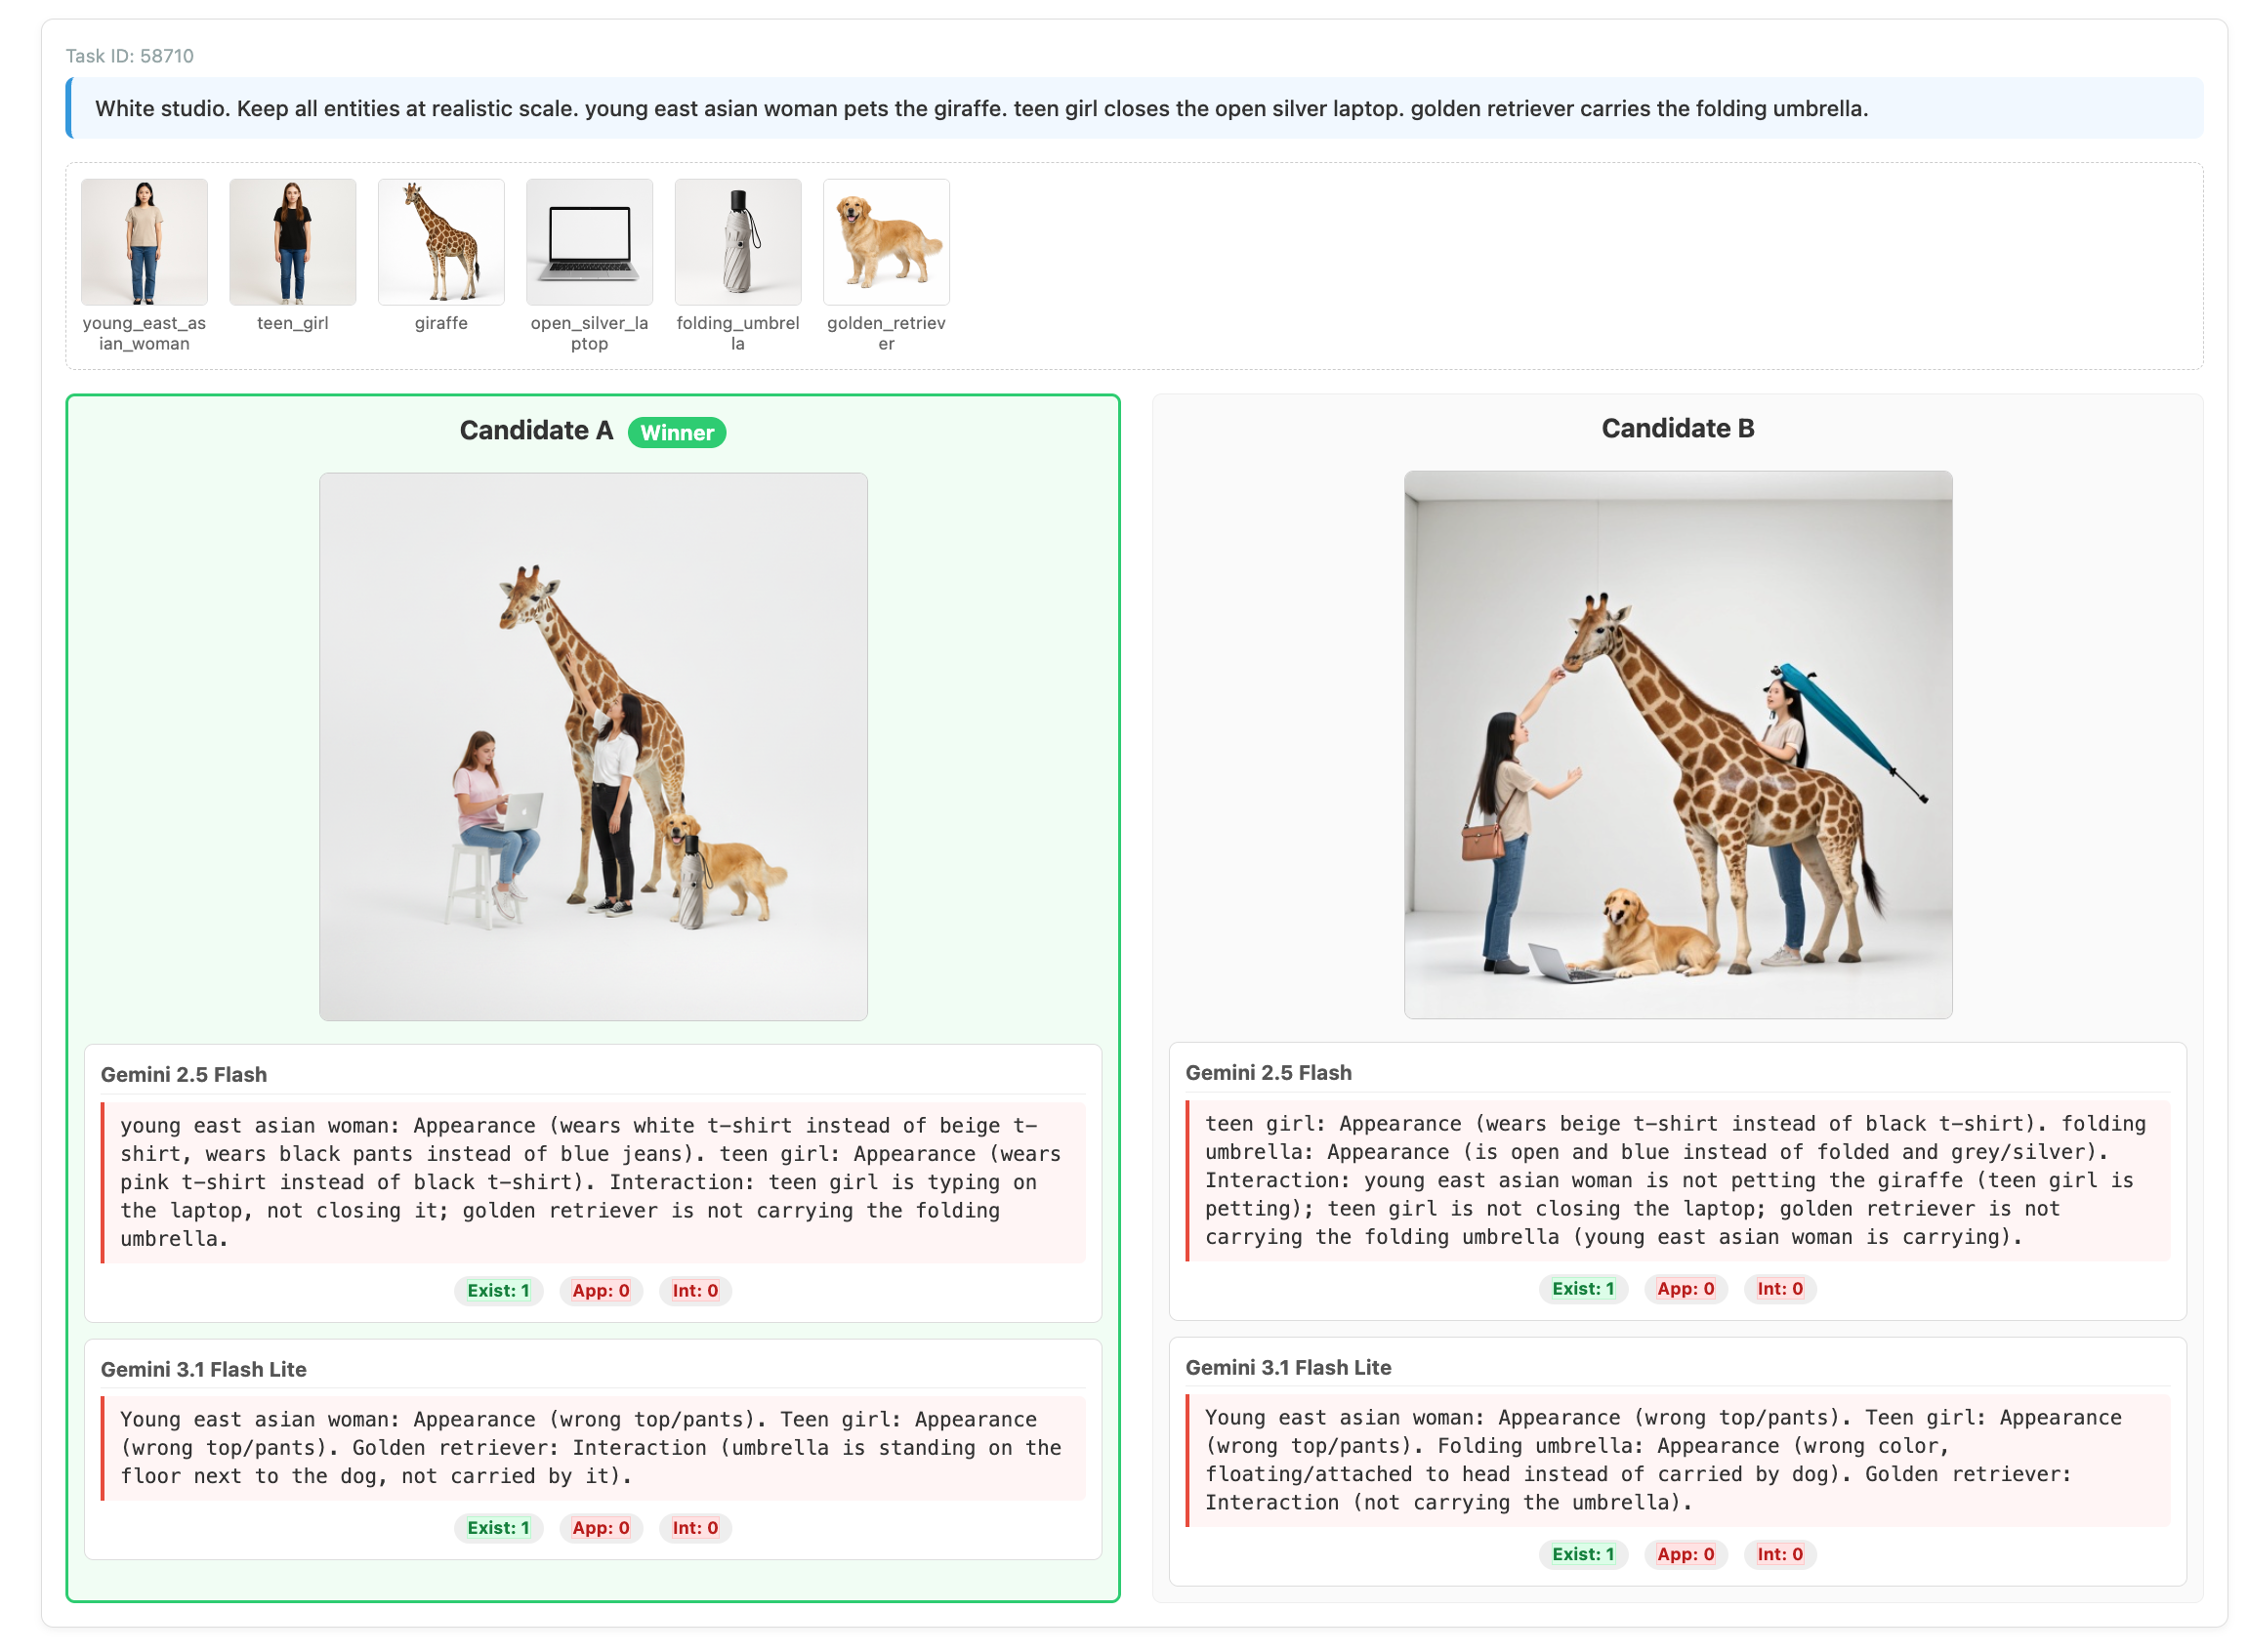
\includegraphics[width=\textwidth]{figures/SOP_demo_5.png}
        \caption{Robust Diagnostics in Highly Complex (6-Subject) Scenes}
    \end{subfigure}
    \caption{Qualitative examples of strict cross-model consensus. The externalized flaw logs demonstrate that both VLMs effectively utilize the SOP to catch fine-grained errors in appearance, physical realism, interaction semantics, and complex multi-subject scaling.}
    \label{fig:sop_demos}
\end{figure}


\newpage
\input{checklist}
\end{document}
